% (C) Anders Kofod-Petersen
\raggedbottom
\documentclass[b5paper, twoside, titlepage, 10pt]{report}
\setcounter{secnumdepth}{3}
\usepackage[lmargin=25mm,rmargin=25mm,tmargin=27mm,bmargin=30mm]{geometry}
%\documentclass[11pt, b5paper]{report}
\usepackage[english]{babel}						% Correct English hyphenation
\usepackage[utf8]{inputenc}						% Allow for non-English letters
\usepackage{graphicx}							% To include graphics
\usepackage{natbib}								% Correct citations
%\usepackage{fancyheadings}						% Nice header and footer
\usepackage[linktocpage,colorlinks]{hyperref}			% PDF hyperlink
%\usepackage{geometry} 							% Better geometry
\usepackage{import}
\usepackage[toc,page]{appendix}
\usepackage{tabularx}
\usepackage[section]{placeins}
\usepackage{mathtools}
%\usepackage{amsmath}
\usepackage[]{algorithm2e}
%\usepackage[center]					% For cropping documents
\usepackage{titlesec}
\usepackage[usenames,dvipsnames]{xcolor}

\usepackage{float}
\setcitestyle{square}


% spacing: how to read {12pt plus 4pt minus 2pt}
%           12pt is what we would like the spacing to be
%           plus 4pt means that TeX can stretch it by at most 4pt
%           minus 2pt means that TeX can shrink it by at most 2pt
%       This is one example of the concept of, 'glue', in TeX

\titlespacing\section{0pt}{10pt plus 4pt minus 2pt}{10pt plus 2pt minus 2pt}
\titlespacing\subsection{0pt}{8pt plus 4pt minus 2pt}{8pt plus 2pt minus 2pt}
\titlespacing\subsubsection{0pt}{6pt plus 4pt minus 2pt}{6pt plus 2pt minus 2pt}

% B5 (uncomment to convert to B5 format)
%\geometry{b5paper}

% Author
% Fill in here, and use commands in the text. 
\newcommand{\thesisAuthor}{Hanne Gunby and Susanne Gustavsen}
\newcommand{\thesisTitle}{\color{Magenta} The Fairy Tales of the Ant Princesses}
\newcommand{\thesisType}{Masters Thesis}
\newcommand{\thesisDate}{Spring 2014}

%Fancy headings
%\pagestyle{fancy}
%\pagestyle{fancyplain}
%\renewcommand{\chaptermark}[1]{\markboth{#1}{}}
%\renewcommand{\sectionmark}[1]{\markright{#1}{}}
%\lhead[\fancyplain{}{\thepage}]{\fancyplain{}{\let\uppercase\relax\leftmark}}
%\rhead[\fancyplain{}{\let\uppercase\relax\rightmark}]{\fancyplain{}{\thepage}}
%\chead[\fancyplain{}{}]{\fancyplain{}{}}
%\lfoot[\fancyplain{}{}]{\fancyplain{}{}}
%\cfoot[\fancyplain{}{}]{\fancyplain{}{}}
%\rfoot[\fancyplain{}{}]{\fancyplain{}{}}



\begin{document}

\pagenumbering{arabic}
%Title page (This is generate automatically from the commands above)
\begin{titlepage}
\noindent {\large \textbf{\thesisAuthor}}
\vspace{2cm}

\noindent {\Huge \thesisTitle}
\vspace{2cm}

\noindent \thesisType, \thesisDate 
\vspace{2cm}

\noindent Artificial Intelligence Group\\ Department of Computer and Information Science\\ Faculty of Information Technology, Mathematics and Electrical Engineering\\

\vfill

\begin{center}


\includegraphics[width=3cm]{assets/logo_ntnu_eng.pdf}

\end{center}

\end{titlepage}

\cleardoublepage

\section*{Abstract}
%The abstract is your sales pitch which encourages people to read your work but unlike sales it should be realistic with respect to the contributions of the work. It should include:
\begin{itemize}
\item the field of research
\item a brief motivation for the work
\item what the research topic is and
\item the research approach(es) applied. 
\item contributions
\end{itemize}

The abstract length should be roughly half a page of text --- without lists, tables or figures.  


This thesis 
\clearpage
\section*{Preface}
The preface includes the facts - what type of project, where it is conducted, who supervised and any acknowledgments you wish to give.
\clearpage

%content
\listoftables
\listoffigures
\tableofcontents

\chapter{Introduction}
\label{introduction}
AtB is responsible for planning, ordering and marketing public transport throughout Sør-Trøndelag county.


\section{Background and Motivation}

Trondheim and neighboring municipalities are among the areas with the greatest population growth in Norway \citep{website:miljopakken}. More people means more traffic, and without action will congestion and environmental problems increase every year. 

Private transportation have many advantages for the citizens compared to the public ones. They do not have to wait for a vehicle at the beginning of a trip, change vehicles during the trip, and it is often more convenient. The negative issues of private transportation, such as traffic jams and increased travel times, means increased air pollution, noise and accidents. 

Having efficient public transportation systems can substantially reduce negative effects of private transportation networks 
\citep{kechagiopoulos14} . The environment package \citep{website:miljopakken} for transport in Trondheim involves providing better road networks and public transport. With this they hope to achieve lower emissions, shorter traffic jams and less traffic noise. Inadequately designed transit network can cause very long waiting times and increase uncertainty in bus arriving time \citep{nikolic14}. Therefore, public transportation systems should be improved by providing better travel services, and inform the public about them, in order to convince more people to travel with it instead of using their own car. 

 \citet{website:atb} is responsible for planning the public transport throughout Sør-Trøndelag County, and bus services comprise the major component of the public transportation system. Bus services also has specific attractive features, such as flexible routes, medium capacity, low cost (of capital and running), easy implementation, flexible fleet size (easy to expand or contract this size), and use of existing facilities (roads and streets). From a meeting with AtB we learned that the current solution of AtB consists of an experience based route network, where no common methodology is used, and where all bus route networks and schedules are designed manually. As a result, the efficiency of the resulting networks is highly dependent of the designers expedience and his / hers knowledge of existing resource constraints and transportation demands.

 Satisfying all customer needs, and keeping all operator costs in check, is really difficult to achieve \citep{kechagiopoulos14}. Operator costs mainly refer to the total number of buses, total bus running distance and the total operation hours. A minimum trip time, amount of transitions, and a not too crowded bus (customers can tolerate standing in 15 minutes ) are among the most important factors that determine the passengers choice of public transit, AtB experiences.  
 \textit{The main concern of bus companies is maximizing its profits, while the main concern of the government is to fulfill all needs of traveling in public} \citep{kechagiopoulos14}. The manual attempts to provide an acceptable solution this problem are not able to solve these large network problems efficiently \citep{kechagiopoulos14}. 





















\section{Goal and Research Questions}
%TODO: skrive et mer utfyllende avsnitt
\textbf{Goal:}
\begin{itemize}
\item \label{itm:goal} Increase the number of public transportation passengers by making urban transit networks more efficient.
\end{itemize}
\textbf{Research Questions:}
\begin{enumerate}[label=\textbf{\arabic*})]
\item \label{itm:1}
    \begin{enumerate}
    \item \label{itm:1a} Is swarm intelligence methods suitable for the vehicle routing problem?
    \item \label{itm:1b} What is the state-of-the-art in solving vehicle routing problems using swarm intelligence methods?
    \item \label{itm:1c} What changes have been done to the classical swarm intelligence-methods to improve them?
    \item \label{itm:1d} Have there been any attempts to combine different swarm intelligence-methods?
	\end{enumerate}
\item
    \begin{enumerate}
    \item \label{itm:2a} Is it efficient to combine attributes from different swarm intelligence-methods to solve the vehicle routing problem?
    \item \label{itm:2b} Is it possible to apply the proposed algorithm to optimize bus routes in urban cities?
    \end{enumerate}

\item
	\begin{enumerate}
	\item \label{itm:3a} What are the potential advantages and disadvantages of using a graph database in our implementation?
    \end{enumerate}
\end{enumerate}
\section{Research methods}

%What methodology will you apply to address the goals: theoretic/analytic, model/abstraction
%or design/experiment? This section will describe the research methodology applied
%and the reason for this choice of research methodology.

In this thesis, two research methods are applied. The first research method used is a structured literature review, introduced by \citep{kofod2014}. This research is conducted in order to establish the state-of-the-art of using swarm intelligence methods and graph databases to solve Vehicle Routing Problems. The results of the final synthesis are presented as the related work that further forms the basis for the proposed problem statement. 

The second research method is the design and development of the proposed system. Experiments comparing the proposed system to a generic ACO algorithm and several published methods are conducted. To ensure a sufficient comparison basis, the proposed system use a well-known benchmark problem.  

The proposed system also attempts to solve larger problems than the benchmark problem described above. By larger problems, we mean a network with a realistic number of bus stops, roads and routes in the route set. This will establish whether the proposed system supports larger networks, which further allow us to discuss the possible usability in a real urban city. 

For all the experiments, numeric values of established performance criteria, including average travel time, are presented. These values are further used to discuss the performance of the proposed system

%The comparison will be based on the numeric values of well-established performance criteria, such as average travel time experienced by each passenger.

%Experiments comparing the proposed system to other methods described in literature will be conducted. This is done

%In order to answer \vref{itm:RQ1} a Structured Literature Review, as described by \citep{kofod2014}, is conducted. This is done to ensure that we are able to draw valid conclusions about what the state-of-the-art is. The results of the final synthesis is described in Related Work, and this is the basis for the problem statement.

%The research method that is used in order to answer \vref{itm:RQ2} and \vref{itm:RQ3}, is designing the proposed system and conducting relevant experiments. 

%In order to test whether or not the added attributes from other swarm intelligence algorithms is efficient, the performance of the proposed algorithm and generic ACO algorithm is compared. 

%To establish how the proposed system performs compared to other methods described in literature, experiments solving a well-known benchmark problem with the proposed system is conducted. 

%In order to test if the proposed system is applicable for optimizing the transit routes in large urban cities, the proposed system will be tested with larger networks as input. 



\section{Thesis Overview}

DENNE SKAL VI SKRIVE TIL SLUTT

\begin{itemize}
\item What does this thesis contain
\item Give results in a general way
\end{itemize}

This section provides the reader with an overview of what is coming in the next
chapters. You want to say more than what is explicit in the chapter name, if
possible, but still keep the description short and to the point.

\chapter{Background and Motivation}
\label{backgroundAndMotivation}
%This chapter contains the background information about vehicle routing problems and swarm intelligence. Section xx covers the motivation behind the thesis. 
\section{Background Theory}
%TODO: Kanskje skrive litt om hva vi slags bakgrunnsteori vi skal presentere og hvorfor
\section{Vehicle Routing Problem }
%ToDO: Skal denne være med?
Routing problems are represented by relevant locations in a graph. This graph consist of a set of nodes and a set of edges, and is formulated as follows; G = (V,E). They can be distinguished according to the type of requests that need to be serviced, that is either arc-based and node-based routing problems. The vehicle routing problem (VRP) is a node based routing problem, as these problems arise if customers are located at nodes so that vehicles remain at the same position while servicing a customer request\citep{vehiclerouting}.

The Vehicle Routing Problem (VRP) was first introduced by \citet{dantzig59} and is a generic name given to a broad class of optimization problems. It can be described as the task of designing the optimal set of routes for a fleet of vehicles, in order to serve a given set of customers. The problem involves making deliveries to a set of customers with known demands on routes originating and terminating at one or more depots, and the objective is to minimize the total route cost. 

\subsection{Urban Transit Network Design Problem}

The problem of designing urban transit routes and schedules is called the urban transit network problem (UTNDP), and is a sub-problem of the vehicle routing problem. The aim is to design efficient urban transit routes and schedules on an existing transit network with predefined pick-up and drop-off points, such as bus routes. The two major components of UTNDP is called the urban transit routing problem (UTRP) and the urban transit scheduling problem (UTSP).

\begin{itemize}
\item UTRP is the task of developing a set of routes on an existing urban transit network, following certain constraints. It can be defined as the \textit{physical} design of the UTNDP \citep{fan09}. 
 
In a transit network, neighboring nodes (bus stops) are linked by an arc or edge. In the tour planning process a set of (requests / nodes ) needs to be assigned to a set of resources. Performing the assignment and sequencing tasks results in a tour for each vehicle. Each step in a tour, traveling from one request / node to the next, is called a route. A tour plan consists of several routes; several nodes connected by edges. When all the routes in a tour plan are superimposed / layered, this will a form a route network, and is also denoted as the solution of the considered problem. The generation of a tour plan is defined by the objective function, and assigns a specific objective function value to each solution. The goal is to find the optimal solution; the ones with the best objective function among all feasible solutions. \citep{vehiclerouting}. A route network should contain all the nodes, but may not contain all the edges present in the original transit network.

(Accurate estimates of travel demand are essential, and a good tour plan will ensure that travel requirements with a heavy demand are satisfied, with short travel and few vehicle transfers. (Future work: Travel demand can be estimated by examining ticket sales, carrying out a survey, or undertaking analysis. This is difficult in practice, because demand is dynamical and highly sensitive to factors such as pricing and quality of service. In addition to satisfying customer demand, design guidelines are determined by many additional factors, including the street environment and management policies by the local government).)

%TODO: skrive om 
\item UTSP involves the development of schedules, arrival and department times, for the public vehicles, to travel along predefined routes. It can also be defined as the \textit{operational} design of the UTNDP \citep{fan09}. 
The contents of the schedule involves minimizing the time a passenger has to wait at each node (bus sop), within certain constraints, such as limited fleet size and bus capacity.  The total waiting time includes the waiting time at their origin and the sum of transferring time. 

\end{itemize}

UTRP and UTSP are usually implemented sequentially, because the development of routes should be completed before the development of schedules. 

\subsubsection{Difficulties in Solving the UTNDP}
%TODO: flette dette inn i motivation? Skrive om.
There are some difficulties in solving the UTNDP. First of all, the UTNDP is an NP-hard problem due to the need to search for optimal solutions from a large number of possible solutions. Some of the constraints can be difficult to model and satisfy, as the feasibility of the tour plan needs to be ensured, which can involve a significant number of computations. Parts of the solutions are independent, because a performance of a route is dependent on the other routes in the tour plan. Travel demand can be difficult to get hold of and can be different at every hour of the day, and designs will therefore be flawed if the data is of poor quality. In addition, passengers can become confused or dissatisfied if there are to many changes to travel routes different times of day, AtB says. 

%ToDo: skrive om
The ideal situation would be to solve UTNDP in one go, and produce a route network and an associated set of vehicle frequencies simultaneously. But in practice, the nature of a route network means that, once established, it is much more stable and difficult to change than a vehicle schedule. Since travel demand varies, it is easy to schedule more buses at busy times. The level of service requirements is sensitive factors (passenger flow, weather and road conditions), and needs to be adjusted to different situations. Therefore, the quality of the network design may be adversely influenced if transit route network and frequencies are simultaneously optimized. 





\section{Swarm Intelligence}

Swarm behavior is found in many different species in nature, including fish schools and flocks of birds. Many of the species that practice swarm behavior does this because of a biological need to stay together. An example of this is that predators usually attacks one individual, and not an entire flock. This swarm behavior is also found in social insects like ants, wasps, bees and termites. They collaborate on tasks including building nests, gather food and organizing production. These social insect colonies have shown us that simple organisms can perform complex tasks by interacting with each other. The colonies are highly distributed and self-organized, and they adapt well to changes in the environment. Swarm intelligence \citep{beni89} is a branch of artificial intelligence that is strongly influenced by the swarm behavior found i nature, and it tries to adapt these characteristics in intelligent computer systems.

\subsection{Ant Colony Optimization}
In nature ants have proven to be extremely capable of finding an optimal or close to optimal route from the nest to a food source \citep{deneubourg90}. Ants communicate by leaving a pheromone trail that other ants are capable of smelling and follow by a certain probability. Most ant species leave a pheromone trail when retuning to the nest from an important food source, and the ants who decides to follow the same path also leave behind a pheromone trail. The more pheromone units on the trail (i.e. the more ants who choose the given path), the greater the probability the other ants will chose it. Because pheromone disappear over time, shorter paths will be favored over longer paths simply because shorter paths (usually) takes shorter time, and thus will have more pheromone units. 

Ant Colony Optimization (ACO) is a class of graph representation based metaheuristic algorithms designed to optimize routing problems. The first description of an ACO algorithm, called Ant System (AS), was initially proposed by \citet{dorigo96}. The AS strategy developed by Dorigo tries to simulate the behavior of real ants, but he adds several artificial characteristics including visibility, memory and discrete time. \citet{nanda11} described a generic implementation of the algorithm as follows: \\

\begin{algorithm}[H]
 initialize\;
 \While{stop criteria are not met}{
  \ForAll{ants a in A}{
   position a in StartNode
  }
  \Repeat{every ant has a solution}{
   \ForAll{ants a in A}{
    choose nextNode\\* 
    $pheromone_{(currentNode,nextNode)}+=update$
   }
  }
  \ForAll{edges e in B}{
   $pheromone_e += deposit$
  }
  \ForAll{edges e in E}{
   $pheromone_e -= evaporation$
  }
 }
 \caption{Generic Ant Colony Optimization Algorithm}
\end{algorithm}

The idea of ACO algorithms is to create a decentralized system with multiple agents. The agents influence each others decisions using pheromones. In the beginning, before any distinct pheromone trail is laid, the ants choices are random and thus they perform a broad search in the environment. This randomness will decrease over time as the pheromone trails becomes more distinct. The literature describes many different algorithms that can be classified as ACO algorithms \citep{salehi-nezhad07,tripathi09,jiang10, dias14}, and most of authors describes artificial ants with additional features to those found in nature, including vision and memory. The addition of features is typically done to increase the performance of the algorithm and reduce some of the randomness in the beginning.  

%TODO: SKRIVE OM ACO I RUTEOPTIMALISERING! 

\subsection{Bee Colony Optimization}
As described in \citet{lucic03}, bees are capable of performing a variety of complex tasks. One of these tasks are the collection and processing of nectar, which may be considered as extremely organized. The idea is that a bee that leaves the hive to gather nectar, flies to the hives so-called dance floor. The bees that have already found a good food source performs a ``dance'' at the dance floor to advertise that they have found a satisfying source of food. The bee that just came from the hive chooses one of the dancing bees and flies with it to its food source. As stated in \citet{lucic03} the mechanism of deciding which bee to follow is not well understood, but it is considered that ``the recruitment among bees is always a function of the quality of the food source''. After the bee has gathered and returned the food to the hive, the bee has three options\citep{lucic03}:

\begin{enumerate}
  \item It can abandon the food source and return to the dance floor, and again become an uncommitted follower
  \item It can continue to gather nectar from the food source without recruiting nestmates
  \item It can return to the dance floor and dance, and thus recruit nestmates before returning to the food source
\end{enumerate}

Bee Colony Optimization (BCO) is metaheuristic methods, that like ACO, aims to create a decentralized optimization system with multiple agents, based on graph representation. The idea is to apply the collective intelligence of the food gathering process to an optimization system. Like a typical ACO algorithm, a typical BCO algorithm is inspired by the way bees acts in nature, but some of the features of natural bees are added to and removed from the artificial bee. \citet{nikolic14} describes a BCO algorithm where the artificial bee only has two options after returning from a ``food source'': (1) abandon or (2) recruit. \citet{lucic03} gives the artificial bees attributes such as memory and perfect knowledge about the quantity of nectar collected by other bees. Modifications like these can make the algorithms more efficient, and thus more suitable of performing complex combinatorial problems, like the Traveling Salesman Problem. 


\subsection{Particle Swarm Optimization}
%[TODO]: Skrive om PSO


%Kanskje kommentere noe om at det virker vanskelig å bestemme parametere for metaheuristic -> Skrive om metaheuristic? 

\section{Graph databases}
\label{sec:graphdb}
A graph database management system (graph database) \citep{robinson13} is a database management system based on graph theory. The term graph theory has been used in centuries and was first introduced by the Swiss mathematician Leonard Euler (1707-1783). In 1736, he proved that there does not exist a closed walk that crossed exactly once each of the seven bridges of the river Pregel in Köningsberg, now called Kaliningrad \citep{alexanderson06}. Figure \vref{fig:7bridgesEuler} shows Euler's original drawings from his paper written in 1736 \citep{euler1741} of the bridges in Köningsberg. 

\begin{figure}[H]
  \centering
  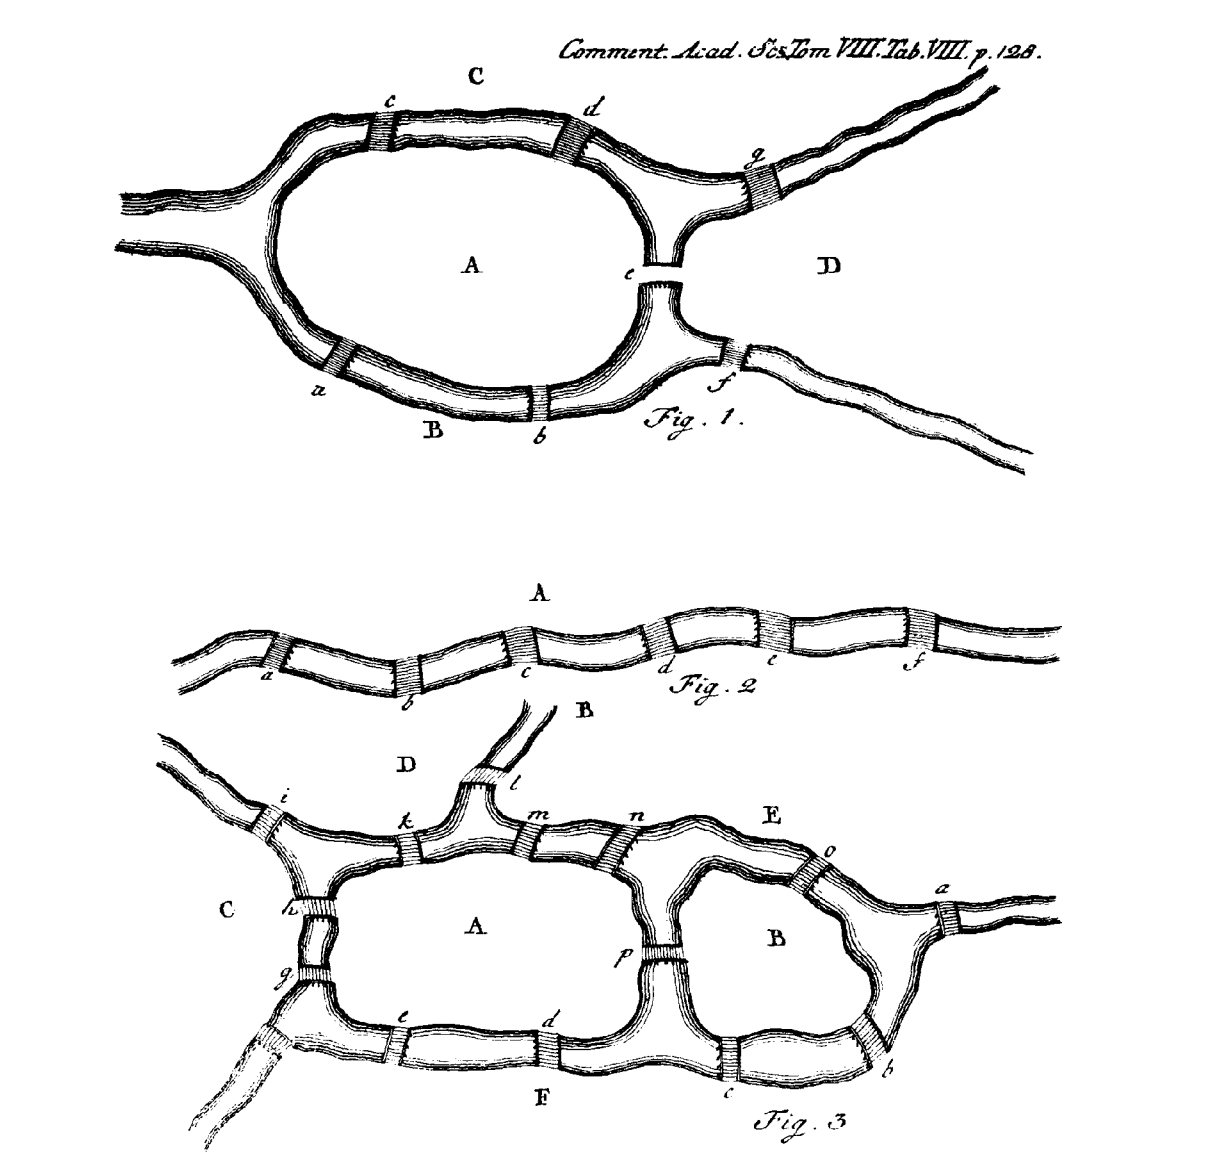
\includegraphics[width=3in]{assets/7bridges-euler.png}
  \caption{Eulers original drawing of the Seven Bridges of Köningsberg} 
  \label{fig:7bridgesEuler}
\end{figure}

%Based on the solution of the ``Seven Bridges of Köningsberg''-problem, Euler presented a theorem. This theorem states that if the graph is planar and connected, and if \textit{v} is the number of vertices, \textit{e} is the number of edges and \textit{f} is the number of faces\footnote{Regions between edges of a plane graph that does not have any edges in it}, then 
%\newline
%\newline
%\centerline{$v-e+f=2$}
%\newline
%\newline
%This theorem demonstrates that if it does not exist a path in the graph that will allow to visit every node using every edge exactly once, the sum will not be 2. An illustration of the bridges in Köningsberg as a graph is presented Figure \vref{fig:7bridgesIllustration} and simplified the illustration in figure \vref{fig:7bridgesSimplification}. The graph consists of 4 vertices, seven edges, and four faces, where the faces are specified with numbers 1-4. If the theorem described above is used, we see that $4-7+4\neq2$, which is consistent with Euler's proof from 1736. 

%\begin{figure}[H]
%  \centering
%  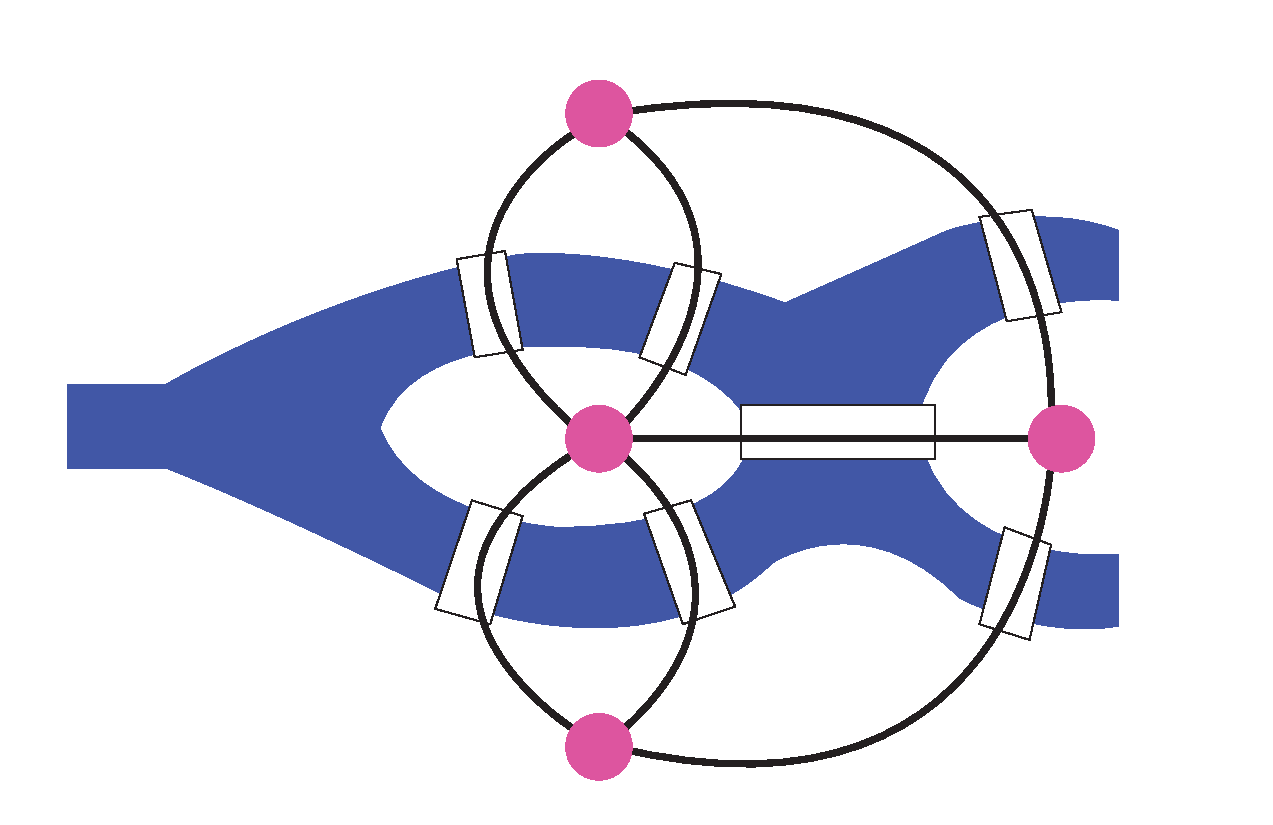
\includegraphics[width=4in]{assets/7bridges.pdf}
%  \caption{Illustration of the Seven Bridges of Köningsberg as a graph}
%  \label{fig:7bridgesIllustration}
%\end{figure}

%\begin{figure}[H]
%  \centering
%  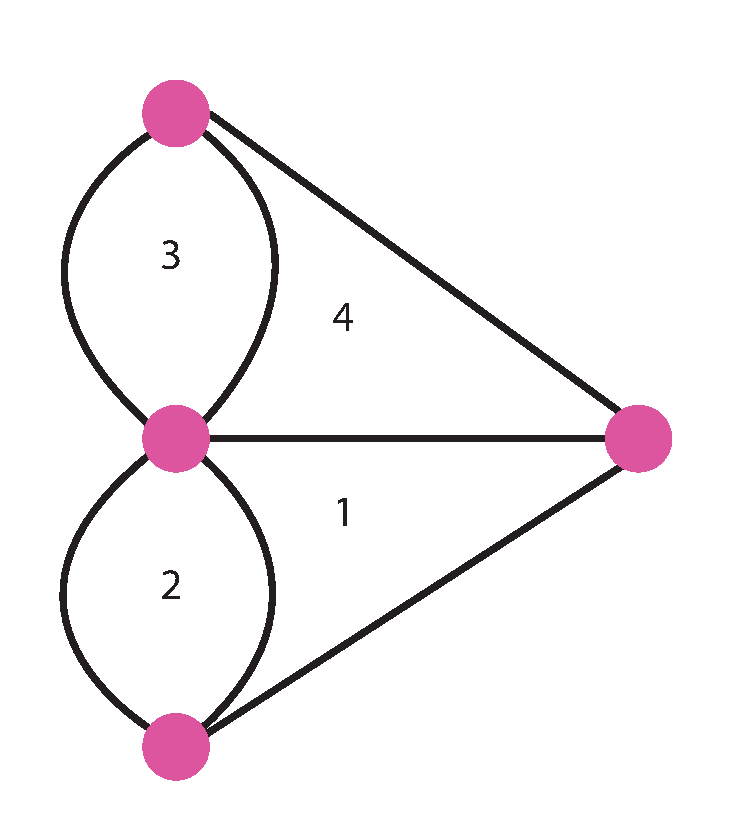
\includegraphics[width=2in]{assets/7bridges2.pdf}
%  \caption{Illustration of the Seven Bridges of Köningsberg as a simplified graph} 
%  \label{fig:7bridgesSimplification}
%\end{figure}

Graph databases use graph structures for semantic queries with nodes, edges, and properties to represent and store data.
The nodes represent entities, such as people, accounts, or bus stops, while the edges represent the relationships, such as ``Friend of'' or ``Belongs to'', between the nodes. A property is relevant information that can relate to either a node or an edge, such as ``Name'' or ``Travel Time''.
%Må omformuleres
Applications of graph databases can include calculating routes and finding the shortest path between locations in a network, such as a road or rail network, airspace network, or logistical network \citep[p.102]{robinson13}. 
%Må omformuleres Compared to relational databases, are graph databases often faster for associative data sets, and map more directly to the structure of object-oriented applications. They can scale more naturally to large data sets as they do not typically require extensive join operations. A drawback to graph databases is the inertia of finding all objects of a specific type.  The following operations are not recommended using graph databases: large, set-oriented wueries, graph global operations and simple, aggregate-oriented queries\citep[p. 40-41]{bruggen14}

\subsection{Neo4j}
\label{subsubsec:neo4j}
Neo4j \citep{website:neo4j} is an open-source graph database, implemented in Java. It is ranked the most popular graph database worldwide \citep{website:graphdbranking} and is used by several large companies such as Telenor \citep{website:telenor}, Walmart \citep{website:walmart} and Cisco \citep{website:cisco}. It is a native graph database optimized and designed for storing and managing graphs and is known for extremely fast traversals of relationship. The underlying data model of Neo4j is the labeled property graph and is one of the most generic and versatile of all graph models\citep[p.73]{robinson13}. This graph data model gives four different fundamental building blocks to structure and store data. These building blocks includes Nodes to store entity information, Relationships to connect nodes to another, Properties for relevant information, and Labels for creating subgraphs.

A query that is extremely well suited for graph databases are queries for finding the paths between different nodes in a graph. Neo4j can be used to see whether a path exists, finding the optimal path, and looking for variability in the path\citep[p. 51]{bruggen14}. Neo4j includes built-in methods for finding the shortest path, including Dijkstra's algorithm. Dijkstra's algorithm \cite[p.658-662]{cormen09} maintains a set $S$ of vertices' whose final shortest-path weights from the source $s$ have already been determined. The algorithm repeatedly selects the vertex $u = V - S$ with the minimum shortest path estimate, adds $u$ to $S$, and relaxes\footnote{Making a change that reduces constraints.} all edges leaving $u$. The running time of Dijkstra's algorithm is $O((V + E)log V)$ and it is guaranteed to find the shortest path\cite[p.~661]{cormen09}. %Dijkstra is one of the best-known algorithms to calculate the shortest weighted path between two points on a graph, using the properties of the edges as a weight or costs. 
The Relationships in a Neo4j database are capable of being of different RelationshipTypes that, among others, enables the built-in Dijkstra to find the shortest path using only specific RelationshipTypes.

%Sweet spot use cases of neo4j: complex, join-intensive queries, path finding queries\citep[p. 51]{bruggen14}. 

%TODO skrive mer her

%Advantages:
%\begin{itemize} 
%\item Flexibility: model, develop and visualize the world as you experience it. Its simply nodes and relationships. 
%\item Performance: Hyper-connectivity at speed. 
%\item Scalability: Scales up and out, supporting tens of billions of nodes and relationships, and hundred of thousands of ACID transactions per seconds. 
%\item Speed: Able to search trough millions of connections per second, with real time queries that stay fast even as your database grows. 
%\end{itemize}

%\begin{itemize}
%\item Native graph database. 
%\item Property graph. 
%\item Made for real time queries. 
%\item Really fast traversals of relations.
%\item Neo4J has an API that supports traversing - finding shortest path - can weight edges, nodes -
%\end{itemize}
%//en korteste vei mellom n og m men max lengde 3
%match p = shortestPath ( (n) - [*...3]--(m)) return p
%(Vekte kanter: Neo44J har et API som støtter traversering, Dijkstras er innebyd ++ som lar deg vekte kanter - hva er raskeste vei ++)

%Neo4J can be used to evaluate routes after the ants have created route sets.
\section{Motivation} 

Trondheim and neighboring municipalities are among the areas with the greatest population growth in Norway \citep{website:miljopakken}. More people means more traffic, and without action will congestion and environmental problems in these urban areas continue to increase every year. 

Private transportation has many advantages for the citizens compared to the public ones. The citizens do not have to wait for a vehicle or change vehicles during a trip, and it is often more convenient. But private transportation has a lot of negative issues, such as traffic jams and increased travel times, which leads to increased air pollution, noise and accidents. 
 
Having efficient public transportation systems can substantially reduce negative effects of the private transportation networks. The public transportation systems is better suited for urban needs, when they can transport more people per time unit than cars, needing much less space. The environment package \citep{website:miljopakken} for transport in Trondheim aims to provide better road networks and public transportation. With this they hope to achieve lower emissions, shorter traffic jams and less traffic noise. An inadequately designed transit network can cause very long waiting times and increase uncertainty in bus arriving time, resulting in less people using the service. Therefore, public transportation systems should be improved by providing better travel services, minimizing the total travel time, and inform the public about them, in order to convince more people to travel with it instead of using their own car.

\citet{website:atb} is responsible for planning the public transport throughout Sør-Trøndelag County, and bus services comprise the major component of the public transportation system here. Bus services also has specific attractive features, such as flexible routes, medium capacity, low cost, easy implementation, flexible fleet size, and use of existing facilities. 
From a meeting with AtB we learned that the current solution of AtB consists of an experience based route network, where transport planners has constructed reasonable bus route networks and schedules entirely manually, following guidelines and exploiting local knowledge. As a result, the efficiency of the resulting networks is dependent of the designers experience and his / hers existing knowledge of constraints and transportation demands. 

The problem of designing the optimal set of routes for a fleet of vehicles, in order to serve a given set of customers, is referred to the vehicle routing problem (VRP). The urban transit network problem(UTNDP) is an example of this broader optimization problem, and is the problem of designing urban transit routes and schedules. The two major components of the UTNDP are the urban transit routing problem(UTRP) and the urban transit scheduling problem (UTSP). UTRP involves the development of efficient transit routes on an existing transit network, with predefined pick-up / drop-off point (e.g bus routes), and UTSP is assigning the schedules for the vehicles. In practice, the two phases are usually implemented sequentially, with the routes determined in advance of the schedules.%Skal denne være med her?

Satisfying all customer needs and in addition keeping all operator costs in check, can be difficult to achieve. Operator costs can include the total number of buses, total bus running distance and the total operating hours. A minimum trip time, amount of transitions, and a not too crowded bus (customers can tolerate standing in 15 minutes ) are among the most important factors that determine the passengers choice of public transit, AtB experiences. 

In the past, transit planners have done reasonable job designing transit networks and schedules without the assistance of scientific tools or systematic procedures, by using their experience and judgment and following established guidelines. Nevertheless, for a really large network it is almost impossible to design an efficient transit route network and bus schedules relying only on past experience and guidelines, because in a large urban area the number of bus routes and bus stops are extremely large. The manual attempts to provide an acceptable solution to the vehicle routing problems are not able to solve these large network problems efficient. In order to overcome this problem, the number of journal publications on vehicle routing problems have increased in recent decades, with the researchers efforts to contribute to the problem.  The increase in researching on these areas is also due to the progress in computational resources, and this has opened new possibilities for modeling more complex routing problems. %These new arising real-world applications provide inspiration for developing new approaches for coordinating complex transportation processes. %Skrives om litt
%In recent years network optimization has become an important field in operational research. Shortest paths, network flows, traffic equilibrium, tsp, vrp, as well as design of an optimal network. Reasons for great interest in network optimization: broad applicability to problemts in pricate entrerprise as well as those in public systems. Networks: changing demands: leads to regurlarly adapted or expanded to meet changing nemands; leads to decision problems than can be supported by network optimization. \citep{mandl79}

%TODO: skrive litt til
Swarm intelligence algorithms has proven to be useful in many vehicle routing problems, and many studies have been done to improve the quality of such problems.
\subsection{Related work}

The related work for this thesis is gathered through a structure literature review. This process is conducted by thoroughly considering what we believe is the most important key words for collecting the most relevant literature concerning our goal, and is properly described in the Experiments and Results-chapter[\ref{experimentsAndResults}], and is entirely explained in the appendix[\ref{appendixA}][\ref{appendixB}]. The literature in this section are the results of the final data synthesis of the structured literature review. \newline

Swarm intelligence algorithms has proven to be useful in many vehicle routing problems, and many studies have been done to improve the quality of such problems. One of the research questions in this thesis is to establish whether it is possible to  solve vehicle routing problems using swarm intelligence and the results of the conducted structured literature will help us establish that. \citet{dorigo97} and \citet{lucic03} are two of the first published papers that confirms this research question by describing methods using swarm intelligence to solve highly complex route optimization problems. The use respectively an ant colony system and a bee system to solve the Traveling Salesman Problem (TSP), which is a subproblem of VRP. 

\citet{hsiao04} presented an optima approach to search for the best path of a map considering the traffic loading conditions. To do this, they proposed an algorithm based on ACO techniques to search for the shortest path from a desired origin to a desired destination. They random-generated a map consisting of 100-500 nodes, and compared their algorithm to a brute method emphasizing on the time used to generate the route. Their results states that if the map consists of more than 200 nodes, the ACO performs better than a brute method. In fact, their results shows that the more nodes the map contains, the higher the benefit of using the ACO algorithm.  

\citet{yang07} presented an optimization model for a bus network design based on the coarse-grain parallel ant colony algorithm (CPACA). CPACA is an optimization algorithm the develops a strategy to update the increased pheromone, called Ant Weight, where the path searching activities of the ants are adjusted based on the objective function. The model aims to minimize the average trip time by maximizing the number of direct travelers per unit length. Their results are compared with the classical MAX-MIN ant system (MMAS)\citep{stutzle99} and with ACA with Ant-weight strategy (ACA+). The comparison shows that CPACA performs better regarding both average direct traveler density and run time. They concluded that suitable future research will be to improve the searching efficiency, because their simulation shows that their algorithms is more stable and the runtime is more satisfactory when the number of nodes are less than 1000. 

\citet{salehi-nezhad07} presented an algorithm to search for the best direction between two desired origin and destination intersections in cities, called Ant-based Vehicle Navigation algorithm. The algorithm was applied on a part of the city of \textit{Kerman}, and the results are encouraging. The algorithm provides a fast access, low cost and easy method for vehicle navigation in cities without assisting GPS.

\citet{tripathi09} solved the vehicle routing problem with stochastic demand, in which the customer demand is modeled as a stochastic variable. They performed this using an improved version of the ACO approach, called ns-AAA SO, which oriented the search progressively towards favoring the global optimal solution. The characteristics and search capability of ns-AAA SO was then compared with both a standard ACO algorithm and a genetic algorithm. The results shows that ns-AAA SO outperforms the other two algorithms in every problem instance described by the authors. 

\citet{salehinejad10} introduced a route selection system which uses an ant colony system to detect an optimum multiparameter direction between two desired points in urban areas. The system employs fuzzy logic for local pheromone updating, and the proposed algorithm is called Fuzzy Logic-Ant Colony System (FLACS). The algorithm is applied to a part of London, United Kingdom, consisting of 42 junctions (nodes). The FLACS algorithm is compared to a standard ACS-algorithm and a $A^*$-ACS-algorithm emphasizing on the parameters ``distance'', ``traffic'' and ``incident risk'', which is said to be important to travelers. The presented results are the average of 10 randomly selected O/D pairs, and their result graphs states that FLACS performs better at average than both the standard ACS and the $A^*$-ACS regarding operational cost. The performance is independent of the importance rate of the parameters mentioned above. It is, however, worth mentioning that the estimation of further traffic data is done by ANNs, and therefore the traffic data used for each algorithm is not exactly the same. FLACS has less running time than $A^*$-ACS, but more than the standard ACS due to its Fuzzy Logic system component. 

\citet{jiang10} describes an improved ACO (IACO) algorithm to solve the Urban Transit Network Optimization which is described as a typical nonlinear combinatorial optimization problem. Improvements to the algorithm includes a stagnation counter to determine if an ant had stagnated and adding of extra pheromone intensity to newly discovered paths. This is done to compensate for the classical ACOs shortcomings of easily falling into stagnation and therefore obtain a local optimal solution. The IACO algorithm is, like the algorithm described by \citet{yang07}, compared to the classical MMAS algorithm. The results shows significant improvement to the convergence speed compared to MMAS. The average number of iterations to find the optimal solution was reduced from 1060 using MMAS to 548 using IACO. The average path distance was shortened from 15554.74 using MMAS to 15509.02 using IACO.  

\citet{poorzahedy11} proposed an Ant System application for solving the bus network design problem. The bus network design problem is a problem that is usually decomposed into two problems, respectively network configuration and bus frequency determination. Some of the characteristics of the authors algorithm is that it works with a decision graph, rather than on the bus network it self. The algorithm is only concerned about one objective; a combination of travel time for the users and the bus fleet size for the operator. The application was used to design the bus network of Mashhad, a city with a population of over 2 millions, and further compared with a genetic algorithm (GA). Their results shows that their algorithm performs better than the GA in both the number of routes, fleet size, in-vehicle travel time and waiting time. GA performs better than the Ant System algorithm with respect to travelers walking time. 

\citet{dias14} introduced an inverted ACO (IACO) algorithm. The idea was that the IACO algorithm inverts the classical ACO logic by converting the attraction of ants towards pheromones into a repulsion effect. The IACO was then used in a decentralized traffic management system, where the drivers acts as the inverted ants. The ideas was that drivers are repelled by the scent of pheromones (other drivers), and the system thus avoids congested roads. The IACO algorithm described, was compared to a shortest-time algorithm (ST). The IACO algorithm performs better than the ST algorithm, with the respect to trip time, travel length, fuel consumption and $CO_2$ emissions. This is as long as a considerable amount (25-50\%, depending on whether it was tested on a radial and ring network or a lattice network) of the vehicles uses an algorithm to decide which road to choose. 

\citet{nikolic14} proposed a model for the transit network design problem. To do this they used an approach based on BCO metaheuristic. They considered the network design problem in a way that the algorithm decided the links that was included in the transit network, and further creating designed bus routes based on the links. They tested two orders of importance of the objective functions (an order that is best for passengers and an order that is best for the transit operator). The algorithm was tested on Mandl's benchmark problem of a Swiss bus network\citep{mandl80}. This is probably the only widely investigated and accepted benchmark problem in the relevant literature\citep{kechagiopoulos14}. Their algorithm was compared to other competitive approaches (\citet{mandl80}; \citet{shih94}; \citet{baaj95}; \citet{bagloee11}), and the results may be considered as ambiguous. The algorithm proposed by \citet{nikolic14} performed best regarding travel time and number for transfers, but was sometimes outperformed regarding in-vehicle time and out-of-vehicle time. 

\citet{sedighpour14} introduced a hybrid ACO (HACO) algorithm where they used a new state transition rule and a candidate list, as well as several local search techniques and a new pheromone update rule. The hybrid was designed to overcome some of the original ACOs shortcomings, such as slow computing speed and local convergence. The HACO algorithm was applied to the open vehicle routing problem, a variant of the vehicle routing problem in which vehicles are not required to return to the depot after completing a service. The HACO algorithm was compared with three versions of PSO (standard PSO, PSO without one-point move (PSOWO) and PSO without neighbors (PSOWN). The algorithms were tested on fifteen different sets, consisting of 19 to 72 nodes with 2 to 7 vehicles fixed at the minimum possible. Their result table showed that HACO found the optimal solution in 14 out of 15 set compared to PSO with 13/15, PSOWO with 0/15 and PSOWN with 9/15. In the one set HACO did not find an optimal solution it still performed better than the other algorithms. As mentioned above, HACO was designed to overcome some of the original ACOs shortcomings and we therefore believe it is worth mentioning that the algorithm was not actually compared to the original ACO algorithm. 

\citet{kechagiopoulos14} designed and presented an optimization algorithm based on PSO. Their goal was to find an efficient solution to the urban transit routing problem (UTRP), which is a NP-hard problem that deals with the construction of route networks for public transportation. The target problem was Mandl's benchmark problem. Their algorithm is compared with competitive approaches (including genetic algorithms and other metaheuristic approaches) mentioned in literature (\citet{baaj91}; \citet{chakroborty02}; \citet{kidwai98}; \citet{fan10}; \citet{fan09-2}; \citet{zhang10}; \citet{chew12}). The algorithms are compared with regard to the percentage of total transfer demands satisfied directly ($d_0$), with one transfer ($d_1$), two transfers ($d_2$), or with more than two transfers or not satisfied at all ($d_{unsat}$). The algorithms are also compared regarding average in-vehicle travel time ($ATT$). The experiments are conducted on route set designs with four, six, seven and eight routes. The proposed algorithm performs better than the competitors regarding $ATT$ independent the route size, and achieves a better percentage of direct travelers ($d_0$) except from when the route size is four. The percentage of passengers with more than two transfers or not satisfied at all ($d_{unsat}$), is $0.00$ for all the described algorithms independent of route size. \newline

Based on the described literature we can conclude that swarm intelligence-algorithms shows great promise in solving different vehicle routing problems. We specifically notice that SI-algorithms performs equal and sometimes better than genetic algorithms and  metaheurstic approaches like Simulated Annealing. We also notice that 2 out of the 12 described papers uses Mandl's benchmark problem as a test case for their proposed algorithm, and that 2 out of 12 papers compare their algorithm to \citet{stutzle99}s MAX-MIN ant system (MMAS). It is worth mentioning that none of the proposed algorithms performs optimally in every situation and that there is no consensus in which algorithm is the overall best. It is therefore difficult to draw a singular conclusion to what is the state of the art regarding swarm intelligence and vehicle routing problems. We suggest that a general state of the art regarding the algorithm may be described as being inspired by the way different swarms act in nature, and to further add artificial features to the individuals to optimize for certain objectives. Mandl's benchmark problem was used by 2 out of the 4 papers in our literature review published in 2014, and we therefore believe that using this benchmark problem as a test case may be considered as the state of the art.


%Skrive om at det "To the best of our knowledge" ikke eksisterer en supersverm algoritme. 

\subsection{Mandls Benchmark Problem}
%TODO: kjøpe/leie Mandl boka
%TODO: skrive om 
%Since there is not done any op
In the current research on the VRPs and SI, there are some benchmark data that are available for researchers to use for comparison.... However (as mentioned in RW), for the UTNDP problem, Mandls network seems to be the only benchmark instance used by researchers. The road network is a real Swiss road network comprising of 15 nodes and 21 connections between them. And has been thoroughly examined by many optimization approaches such as \citep{kechagiopoulos14}, \citep{fan09}, \citep{nikolic14}. %This makes it easy to measure the performance of your solution. 

%TODO: skrive om 
Christoph Mandl concentrated mainly on the UTRP, and developed a solution in two stages. First, a feasible set of

Christoph Mandl[] approaches the UTNDP problem in a generic form. Mandl concentrated on the UTRP, and developed a solution in two stages. First, a feasible set of routes was generated, and then heuristics were applied to improve the quality of the initial route set / tour plan. The route generation phase involved computing the shortest path between all sets of vertices's using Dijstras[], and then producing the route set with the shortest paths that contained the most nodes, respecting the positions of any nodes selected as terminals. Nodes not selected, were iteratively included into routes, or new routes were created with unserved nodes as route terminals. In the first phase, Mandl only considered in-vehicle travel costs when accessing route quality. He then suggested an initial route set, and used these in the second phase. The second phase included obtaining the new routes at an intersection node, including a node that was close to a route (if travel demand between this node and the node on the route was high), and / or excluded a node from a route set that was already served by another rote (if the travel demand between this node and the other nodes in the route was low). Waiting costs were also considered in the second phase, in addition to in-vehicle travel costs. Waiting times were fixed as constant values, according to specified vehicle frequencies. 

%IFylles inn i results: in order to demonstrate the efficiency and the effectiveness of our algorithm... the Swiss road network introduced by Mandl is used. This road network has been already used as a benchmark problem by many researchers in the literature. \citep{kechagiopoulos14}


\subsection{Graph Database}
\textit{Denne er foreløpig kopiert fra Wikipedia}
%Skrives om
\par
A graph database is a database that uses graph structures for semantic queries with nodes, edges, and properties to represent and store data. A graph database is any storage system that provides index-free adjacency.This means that every element contains a direct pointer to its adjacent elements and no index lookups are necessary. General graph databases that can store any graph are distinct from specialized graph databases such as triplestores and network databases.
%Skrives om
Graph databases are based on graph theory. Graph databases employ nodes, properties, and edges. Nodes represent entities such as people, businesses, accounts, or any other item you might want to keep track of. Properties are pertinent information that relate to nodes. Edges are the lines that connect nodes to nodes or nodes to properties and they represent the relationship between the two. Most of the important information is really stored in the edges. Meaningful patterns emerge when one examines the connections and interconnections of nodes, properties, and edges.

Compared with relational databases, graph databases are often faster for associative data sets[citation needed], and map more directly to the structure of object-oriented applications. They can scale more naturally to large data sets as they do not typically require expensive join operations. As they depend less on a rigid schema, they are more suitable to manage ad hoc and changing data with evolving schema's. Conversely, relational databases are typically faster at performing the same operation on large numbers of data elements.
Graph databases are a powerful tool for graph-like queries, for example computing the shortest path between two nodes in the graph. Other graph-like queries can be performed over a graph database in a natural way (for example graph's diameter computations or community detection).

\subsubsection{Neo4J}
Neo4J is a native graph database, and is a success way to store a transport graph [Reference]. It is known for extremely fast traversals of relationships. Neo4J can be easily constructed to a transit network. It is fast finding shortest path (by Dijkstra's algorithm), and it is easy to change the database via the REST API. 
Neo4J is a highly scalable open source graph database that supports ACID, has high-availability clustering for enterprise deployments, and comes with a web-based administration tool that includes full transaction support and visual node-link graph explorer. Neo4j is accessible from most programming languages using its built-in REST web API interface. Neo4j is the most popular graph database in use today.[10]


%\begin{itemize}
%\item Native graph database. 
%\item Property graph. 
%\item Made for real time queries. 
%\item Really fast traversals of relations.
%\item Neo4J has an API that supports traversing - finding shortest path - can weight edges, nodes -
%\end{itemize}
%//en korteste vei mellom n og m men max lengde 3
%match p = shortestPath ( (n) - [*...3]--(m)) return p
%(Vekte kanter: Neo44J har et API som støtter traversering, Dijkstras er innebyd ++ som lar deg vekte kanter - hva er raskeste vei ++)

%Neo4J can be used to evaluate routes after the ants have created route sets.
\subsection{Problem Statement}
%TODO: skrive hva vi skal gjøre
Through our review of research, we note that there have been no research that aims to combine attributes from different swarm intelligence methods to improve the optimization process. For this reason, we will in this thesis investigate the possibility to combine some of the best attributes from ACO and BCO in order to achieve better results regarding route optimization.

After a meeting with AtB we learned that AtB does not have accurate data about the travel demand, and that there has not been done any attempts to optimize their transit network with computational resources. Accurate estimates of travel demand are essential as they are an important factor for the algorithm. A good tour plan will ensure that travel requirements with a heavy demand are satisfied, with short travel times and few vehicle transfers. 

We are highly motivated on the development of an algorithm and we want to focus our research on the development of a new algorithm, rather than on gathering data to determine the travel demands of the bus network of Trondheim. In order to demonstrate the efficiency and the effectiveness of our algorithm we will compare our results with Mandls benchmark data. Mandls benchmark problem includes %TODO: FYLL INN SUS%
As mentioned, this road network has already been used as a benchmark problem by many researchers in the literature. We believe that a comparison of our algorithm to others described in literature, will be important to establish both the efficiency and the effectiveness of our algorithm. This comparison will be enabled using Mandls network. Our aim is to create a general solution, where we hope to achieve better results than the ones we are comparing it with, and that this in the future can be used to optimize AtBs transit network. 

We will focus our research on the urban transit routing problem, to make the routes more convenient both concerning customers and operators. The objectives we want to focus on is satisfying the customers and in addition keeping the operator costs in check. Trough our research we have found that 
\begin{itemize}
\item Minimum number of transfers
\item Minimum in-vehicle time
\end{itemize}
is important factors for determine the customers satisfaction ({\citet{kechagiopoulos14}; \citet{dias14}, \citet{yang07} }). There has also been done a lot of research on these areas, and therefore data is available so we can compare our results against this. This factors will also lead to minimum total travel time. 
\par
Minimum fleet size and better departures will implicitly ..
\par
Based on these new routes, we can hopefully draw conclusions....


  


\input{chapters/backgroundTheoryAndMotivation/relatedWorkVol3}
\subsection{Problem Statement}
%TODO: skrive hva vi skal gjøre
Through our review of research, we note that there have been no research that aims to combine attributes from different swarm intelligence methods to improve the optimization process. For this reason, we will in this thesis investigate the possibility to combine some of the best attributes from ACO and BCO in order to achieve better results regarding route optimization.

After a meeting with AtB we learned that AtB does not have accurate data about the travel demand, and that there has not been done any attempts to optimize their transit network with computational resources. Accurate estimates of travel demand are essential as they are an important factor for the algorithm. A good tour plan will ensure that travel requirements with a heavy demand are satisfied, with short travel times and few vehicle transfers. 

We are highly motivated on the development of an algorithm and we want to focus our research on the development of a new algorithm, rather than on gathering data to determine the travel demands of the bus network of Trondheim. In order to demonstrate the efficiency and the effectiveness of our algorithm we will compare our results with Mandls benchmark data. Mandls benchmark problem includes %TODO: FYLL INN SUS%
As mentioned, this road network has already been used as a benchmark problem by many researchers in the literature. We believe that a comparison of our algorithm to others described in literature, will be important to establish both the efficiency and the effectiveness of our algorithm. This comparison will be enabled using Mandls network. Our aim is to create a general solution, where we hope to achieve better results than the ones we are comparing it with, and that this in the future can be used to optimize AtBs transit network. 

We will focus our research on the urban transit routing problem, to make the routes more convenient both concerning customers and operators. The objectives we want to focus on is satisfying the customers and in addition keeping the operator costs in check. Trough our research we have found that 
\begin{itemize}
\item Minimum number of transfers
\item Minimum in-vehicle time
\end{itemize}
is important factors for determine the customers satisfaction ({\citet{kechagiopoulos14}; \citet{dias14}, \citet{yang07} }). There has also been done a lot of research on these areas, and therefore data is available so we can compare our results against this. This factors will also lead to minimum total travel time. 
\par
Minimum fleet size and better departures will implicitly ..
\par
Based on these new routes, we can hopefully draw conclusions....



\chapter{The Model}
\label{theModel}
This is the main structure of what you built.
- Not at code level, but you can include pseudocode.
Explain the system in a way the reader understands it.
Include diagrams and the algorithms used.

\section{Objective function}
\textbf{Reserach Question 2: }

Using Mandl, the constraints and evaluation criteria defined under, we will manage to answer research question number 2: Is it efficient to combine attributes from different swarm intelligence methods to optimize a transit network? This is because we facilitate the comparison with other algorithms results mentioned in the literature. 


\textbf{Initialization}
\begin{itemize}
\item The route size is predefined. The algorithm / routes shall not exceed the minimum or maximum limit of nodes.
\end{itemize}

\textbf{Constraints}
\begin{itemize}
\item A passenger should be able to travel between any two nodes in the route network. In other words, it should be a connected graph. 
\item No cycles (or backtracks) in the graph is allowed.
\item To simplify the problem, there are exactly r routes in the route set.
\item The number of nodes in the routes .... 
\end{itemize}

\textbf{Evaluation criteria}
These will be given higher pheromone
\begin{itemize}
\item Total travel time (should be as low as possible)
\item Number of transfers
\begin{itemize}
\item Number of direct travelers (should be as high as possible)
\item Travelers with one transfer
\item Travelers with two transfers
\end{itemize}
\item Number of unsatisfied customers (should be as low as possible)
\item The nodes with high demand should have higher priority.
\end{itemize}
\section{The Proposed Algorithm}

We started out with implementing the basic ACO algorithm by \citet{nanda11} as described in chapter \ref{backgroundAndMotivation}.

To overcome some of the known limitations of ACO, and to answer our research question: is it efficient to combine attributes from different swarm intelligence algorithms to solve the vehicle routing problem, we have added some features to the basic ACO

\begin{itemize}
\item \textbf{Inertia weight(IW) from PSO}. CrazyAnts: picking a random edge, not based on the pheromone value on the edge. IW his high in the start; more CrazyAnts, but decreases over time (each iteration) resulting in less and less CrazyAnts. This is done to overcome the known limitation of ACO: getting stuck on local optima.
\item \textbf{Global best solution from PSO}. Each iteration, the best ant is retained - and when the next ant is selecting the next edge, the edge of current best ant is added to the probability for this edge to be selected again, resulting in an even greater chance for this edge to be selected.
\item \textbf{Followers from BSO}. 10\% of the ants selects the same routes as the final best ants, and the pheromone value for the edges in these route sets decreases.
\end{itemize}

: SuperSwarm

\subsection{Initialization}
Initial values for algorithm parameters are set to a numeric value. The parameters to be set for this algorithm are:
\begin{enumerate}
\item The ant colony size. 
\item The numbers of iterations (which is the stop criteria).
\item The evaporation constant, $pheromone_{evaporation}$, to determine how much pheromone to be removed at each edge at each iteration.
\item The pheromone constant, $pheromone_{visited}$, to determine how much pheromone to be added to each edge as it is visited by ants.
\item The pheromone constant, $pheromone_{bestRoutes}$, to determine how much extra pheromone to be granted to edges included in the \textit{n} best route sets.
\item The percentage of complete route sets to be granted extra pheromone.
\item Number of routes in a complete route set. 
\item The maximum and minimum number of nodes in the routes.
\end{enumerate}
The value of parameters 1-6 are determined by a conducted experiment described in \ref{subsec:parameterSettings_plan}, \ref{subsec:parameterSettings_setup}, and \ref{subsec:parameterSettings_results} on the pages \pageref{subsec:parameterSettings_plan}, \pageref{subsec:parameterSettings_setup}, and \pageref{subsec:parameterSettings_results}. The value of parameters 7-8 will be the same as the corresponding parameters in \citet{kechagiopoulos14} and \citet{nikolic14} for comparison reasons. 

Further, a network is generated consisting of nodes from the data in the MandlCoordinates file shown in table \ref{table:MandlCoords} on page \pageref{table:MandlCoords} and edges from the data in the MandlDemand file shown in table \ref{table:MandlDemand} on page \pageref{table:MandlDemand}. Travel times are added to the generated edges based on the data in the MandlTravelTimes file shown in table \ref{table:MandlTravelTimes} on page \pageref{table:MandlTravelTimes}. As one can see in table \ref{table:MandlTravelTimes}, some of the travel times are described as ``Inf'', meaning there is no direct path between the two nodes in question even though there is a (possibly) high demand between them. Edges with an ``Inf'' travel time are excluded for the most part of the algorithm, because there is in fact not possible to travel between the nodes connected by the edge. However, when the route sets are evaluated, the algorithm awards sets that satisfy node couples with high demand directly. After this, the generated network is used to create a Neo4j graph database. As stated in research question \ref{itm:3a}, we want to explore the possible advantages and/or disadvantages of using Neo4j in our implementation.



\subsection{Selecting the start node}
The specific steps executed to select the start node of each route are the following:
%Selecting the first node: 
\begin{itemize}
\item[Step 1] The demand value for each node is estimated, which is the sum of each line in the demand table \ref{table:MandlDemand} on page \pageref{table:MandlDemand}. 
\item[Step 2] The nodes is sorted in descending order based on the demand value of each node.
\item[Step 3] The first k nodes from the list is selected, which comprise the initial node set (INS). 
\item[Step 4] Based on the demand value belonging to INS, a probability is assigned to each node, which reflects the probability of each node to be selected as the first node of the route. 
\item[Step 5] A random node is selected based on the values of probabilities. (To prevent a route from having less than the minimum number of nodes, constraint \ref{itm:constraintRouteSize}, it is not possible to select a node with a connected node that only has one edge connected to it.)
\end{itemize}
%Start node for the next ants: Possible hot spots may be detected, and that this can be used as a start node for the next ants. 

\subsection{Selecting the next nodes}
The next nodes is selected based on the demand value, the pheromone value and the visited status value for the edges. \emph{\color{red} A good route network will ensure that routes having the most traveling demands are satisfied with short paths and few vehicle transfers as stated in the problem statement.} The visited status value checks if the node is visited in an earlier route within the same route set. Its value is 0 if it is unvisited, else 1, giving the unvisited nodes a higher probability of being selected. It is only possible to select edges connected by travel time when this indicates whether it is a direct link between the two nodes, but the travel time value is not taken into account before the evaluation phase \emph{\color{red} because..}.  %TODO: give higher score if there is direct routes between node couples with high demand. 
The specific steps executed to select the next nodes of each route are the following:
\begin{itemize}
\item[Step 1] The probability, $P_k$, for the next node to be selected is calculated by adding the pheromone(P), demand(D) and an visited status value (V), and dividing it by the total demand (TD), total pheromone (TP) and the total visited status value for all the connected edges to the node (TV):
$$ P_{k} = \frac{D}{TD} + \frac{P}{TP} + \frac{V}{TV}$$ 

\item[Step 2] After each edge is given a probability, these are added in a range starting from 3, decreasing with the probability value for each edge. 
\item[Step 3] A value between 3 and 0 is then random selected, giving the edges with highest probability a larger range than the others, resulting in a larger probability for this edge to be selected. 
\item[Step 4] After an node is selected, the pheromone value for this edge increases 
\end{itemize}

\subsection{Creating the route set}
The node selecting phase stops if it exceeds $k$ nodes, as constraint \ref{itm:constraintRouteSize} specifies; the route size is predefined, so the routes shall not exceed the maximum limit of nodes. It also stops if it is ``stuck'', because it is should not be possible to select the same node twice, according to constraint \ref{itm:constraintCycles}; no cycles (or backtracks) in the graph is allowed. The ant then begins the next route exploring. The route exploring stops when it exceeds the maximum number of routes, as specified in constraint \ref{itm:constraintRouteSet}; there are exactly $r$ routes in the route set. The routes are then added to the ant's route set for evaluation.

\subsection{Route set evaluation}


\begin{itemize}
\item[Step 1] Only the ants with a connected route set is selected for evaluation. This is important because based on constraint \ref{itm:criteriaConnectedGraph}, a passenger should be allowed to travel from every node to every other node within the route set. In an undirected graph $G$ two vertices $u$ and $v$ are called connected if G contains a path from $u$ to $v$. An ants route set can have included all nodes, but still be disconnected. The ants with a route set that is disconnected is therefore removed from the best ants. The complexity of evaluating this during the route generation stage is the reason this is evaluated after. 

\item[Step 2] This ants are added to the ``best route set'' for evaluation. (Evaluation a route itself as no sense, since its path depends on the rest of the members of the same route set. As a result, all routes of a route set should be evaluated as a whole. This evaluation is based on the evaluation criteria stated in previous section.)

\item [Step 3] The route sets are added to the Neo4J database, and evaluated by a fitness function, TOTFIT(r), where $r$ is the route set, inspired by \citep{kechagiopoulos14}.
This fitness value is calculated as follows:
$$ TOTFIT(r) = F_{1}(r) + F_{2}(r) + F_{3}(r), $$

where $ F_{1}(r)$ is the score obtained by evaluating the route set by the total in-vehicle time, $ F_{2}(r)$ is the score obtained by evaluating the route set using evaluation criteria direct traveler, one transfer, two transfers, and $ F_{3}(r)$ is the score obtained by evaluating the route set using the criteria unsatisfied customers (more than two transfers). 
%$ w_{1}, w_{2}$, and$ w_{3}$ are user specified weights for scores $ F_{1}(r), F_{2}(r),$ and $ F_{3}(r)$, respectively. 
%To find w, we will calculate an average with ratio, and give weights from that, and theese weights sum is 1.  
\end{itemize}

\subsubsection{Calculating $F_{1}(r)$}

This score is obtained by evaluating how good the path between two nodes, $k_1$ and $k_2$, in the route set is. The score is calculated by finding the difference ($DIF$) in travel time between the edges included in the route set, and the actual minimum travel time (shortest path):

$$ DIF = TT(k_{1},k_{2}) - MTT(k_{1},k_{2})$$

where $ TT(k_{1},k_{2})$ is the travel time using the edges included in the route set, and $ MTT(k_{1},k_{2})$ is the actual minimum travel time (shortest path) between the two nodes, regardless of the edges included in the route set. Calculating the minimum travel time (shortest path) is done by Neo4j, and the selection of which algorithm used is described under.

\paragraph{Calculating the Minimum Travel Time}\mbox{}\\ 

Neo4j includes two built-in algorithms for finding the shortest path, including A* search\citep{russel10}  and Dijkstra's algorithm\citep{cormen09}. 

A* search\cite[p.93-94]{russel10} evaluates nodes by combining $g(n)$, the cost to reach the node, and $h(n)$, the cost to get from the node to the goal.

$$ f(n) = g(n) + h(n).$$
Since g(n) gives the path cost from the start node to node $n$, and $h(n)$ is the estimated cost of the cheapest path from $n$ to the goal, we have
$$f(n) = \text{estimated cost of the cheapest solution through $n$} $$ 

A* search is both optimal and complete, provided that $h(n)$ is admissible\footnote{It never overestimates the cost to reach the goal.} or consistent\footnote{When estimating the distance of a given state to a goal state, it is always at most equal to the estimated distance from any neighboring vertex plus the step cost of reaching that neighbor.}. 

$$ \text{A* search running time: } O(E) = O(b^d)$$
\textit{where $b$ is the branching factor (average number of successors per state)}

Dijkstra's algorithm \cite[p.658-662]{cormen09} maintains a set $S$ of vertices's whose final shortest-path weights from the source $s$ have already been determined. The algorithm repeatedly selects the vertex $u = V - S$ with the minimum shortest path estimate, adds $u$ to $S$, and relaxes\footnote{Making a change that reduces constraints.} all edges leaving $u$.

Dijkstra's algorithm is guaranteed to find the shortest path\cite[p.~661]{cormen09}.
$$\text{Dijkstra's algorithm running time: } O((V + E)lg V)$$

\begin{table}[H]
    \begin{center}
        \begin{tabular}{|l|l|l|}
      \hline
      ~ & A* search & Dijkstra's algorithm\\
      \hline
        MIN & 291 & 569 \\
        AVG & 328 & 589 \\
        MAX & 301 & 610 \\
      \hline
        \end{tabular}
    \end{center}
    \caption {A* Search vs. Dijkstra's algorithm}
    \label{table:astarvsdijkstras}
\end{table}

Table \ref{table:astarvsdijkstras} presents the running times for the different algorithms, in seconds, after 20 runs, with 100 iterations, 100 ants, 4 routes,  and max 8 nodes in each route. Observations shows that A* search is faster, \emph{\color{red} because blabla}, and this method is therefore chosen for finding the shortest path in $F_1(r)$.
 
% In other words, it reflects the average time spent by each passenger when traveling along a specific route set. Its value is small if the respective average traveling time is big and big is traveling time is small. In order to estimate F1(r), not only the average traveling time has to be calculated, but one also determine whether this value should be considered big or small. 

\subsubsection{Calculating $F_{2}(r)$}
%TODO: skrive om dette
$F_{2}(r)$ score reflects the percentage of passengers traveling from their origin to their destination either directly, making a single transfer, or transferring twice. Calculating $F_{2}$ is done using the following equation \emph{\color{red} -  kechapocholus har gjort noe mer her, sjekk ut dette..}:
$$F_2(r) = 3xd_0(r)+ 2xd_1(r)+ xd_2(r) $$

where  $d_0(r)$ is the percentage of passengers traveling directly, $d_1(r)$ is the percentage of passengers traveling from their origin to their destination making a single transfer, and $d_2(r)$ is the percentage of passengers traveling from their origin to their destination transferring twice. \emph{\color{red}$x=-1$, and represents? Her må det forklares hvorfor $d_0$ ganges med et høyere tall osv.}. The reason the number is negative is \emph{\color{red}coding reasons. } 

%\begin{itemize}
%\item it checks for the node couple in a route, if the route contains both the nodes, then it is a direct traveler
%\item it checks if the node couple is withing 2 routes
%\item it checks if the the node couple is withing 3 routes
%\end{itemize}

%$f_2(r) = (-3) * directCouples + (-2) * oneTransferCouples + (-1) * twoTransferCouples $

\subsubsection{Calculating $F_3(r)$}
%TODO: skrive om dette
$F_3(r)$ is a score which reflects the percentage of unsatisfied passengers, meaning passengers traveling from their origin to their destination where the number of transfers is more than 3, using route set $r$. It is calculated using the following formula:
$$\emph{\color{red}hannee?}$$

\begin{itemize}
\item[Step 5] 50\% of the best ants are added to the final best ants set.
\item[Step 6] The algorithm awards sets that satisfy node couples with high demand directly. Demand value to consideration.
\item[Step 7] Reward the edges in these routes by giving them more pheromone, and is given by:

$$ \tau_{ij} = \sum_{k=1}^{m} \Delta \tau^k_{ij}$$

where $ \Delta \tau^k_{ij} $ is the amount of pheromone laid on route (i,j) by the $k^{th}$ ant and is given by

$$
\Delta \tau^k_{ij} = \Bigg\{
\begin{array}{l l}
\underline{Q} &  \quad \text{if route (i,j) be traversed by}\\
f_k, &  \quad \text{the $k^{th}$ ant (at the current cycle) , }\\
0 &  \quad \text{otherwise}
\end{array}
$$

Q is a number, tested in parameter setting experiments, and $f_k$: the travel time on the edge.

\end{itemize}

\subsection{Pheromone Evaporation}

The pheromone on each edge decrease by $p\%$ after each iteration. 


\subsection{Route set representation}
For the route set representation, a two dimensional array is selected. In the route set representation presented in table \ref{table:routeSetRepr}, route 1 starts from node 14, continues to node 13, and so on. The routes comprise of 8 nodes, as stated before, the total number of routes is specific, set by the bus company due to cost limitations, while the maximum length is usually defines by the user before the execution of the algorithm \citep{kechagiopoulos14}.
\begin{table}[H]
    \begin{center}
        \begin{tabular}{|l| l l l l l l l l|}
      \hline
        Route 1: & 14 & 13 & 11 & 12 & 4 & 6 & 15 & 9 \\
        Route 2: & 1 & 2 & 5 & 4 & 12 & 11 & 10 & 8 \\
        Route 3: & 9 & 15 & 7 & 10 & 8 & 6 & 3 & 2 \\
        Route 4: & 7 & 10 & 14 & 13 & 11 & 12 & 4 & 5 \\
      \hline
        \end{tabular}
    \end{center}
    \caption {Route set representation}
    \label{table:routeSetRepr}
\end{table}


%TODO: skrive om, og gjøre?
%The number of buses is restricted by some number M. Then, a feasible set of edges is to be found, such that the total transportation time according to some descriptive assignment (with waiting times defined by the number of buses M) is minimized. Since the problem is so complex, only a heuristic algorithm seems appropriate. 
%\begin{itemize}
 %\item Each node will not be served by each bus, but each stop must be served by at least one route ( each node must belong to at least one route. ) Because a passenger must be able to reach a stop from any other stop by using a sequence of routes. But even though all nodes is reachable, many cases people will have to change lines to reach their destination, and this means they have to wait for the next vehicle. Therefore the travel time is the sum of transportation time along the lines plus the sum of waiting. (To include waiting time, means that a node is split into as many nodes as there are lines passing through this node, and if the original node belongs to these new nodes, they are connected by arcs denoting the average travel time. )
 %\item Because changing lines is not only time consuming but also inconvenient for the passengers, many people want to find the one with the least changes necessary. This minimum change path can be found in exactly the same way as the shortest path; instead of assigning the real waiting time for each arc denoting a possible change, one assigns a high value to those arcs, such that a is much greater than the transportation time.
%\end{itemize}





\chapter{Experiments and Results}
\label{experimentsAndResults}

%In the first iteration of a standard ACO as described in \citet{nanda11}, 3 out of 4 ants includes all the nodes in the route set. 
%TODO: kjøre algis et visst antall ganger og ta median og gjennomsnitt og divv divv for å finne div

%Trying and failing is a major part of research. However, to have a chance of success you need a plan driving the experimental research, just as you need a plan for your literature search. Further, plans are made to be revised and this revision ensures that any further decisions made are in line with the work already completed.  
This chapter contains the experiments conducted. 
Section x includes what series of experiments are planned and question what the set of experiments aim to answer. 
Section x includes all data - parameters etc, that would allow a person to repeat your experiments.
Section x includes the results.
%Such questions should be connected to your research questions so that in the evaluation of your results you can discuss the results wrt to the research questions.

%CCohen: The purpose of evaluation at this stage is to convince the researcher and the community that studies of a program - independent of their results - are well-designed and complete. Experiment schema's would offer researchers a shorthand to describe their studies.
\section{Development Environment}

The proposed SuperSwarm Optimization algorithm is programmed in Java programming language. Java is chosen because we are most familiar with that language and therefor believe the development time is reduced. Further, Java is one of the most used programming languages world wide, and the possibility of further contributions is enhanced by using Java. An additional benefit is that Neo4j offers a rich set of integration possibilities for Java and that these possibilities are well documented. Nevertheless, compared to languages like C++, Java is often considered slow and memory-intensive \citep{alnaser12}. However, \citet{sestoft10} states that managed languages like Java are easier and safer to use than traditional languages like C++. \citet{sestoft10} concludes, based on his conducted experiments, that ``there is no obvious relation between the execution speeds of different software platforms, even for the very simple programs studied here: the C, C\# and Java platforms are variously fastest and slowest''.

An embedded version of the Neo4j database is used in order to represent the network including nodes, edges and the created routes. Because we have many reads and writes to the database, an embedded version is preferred because it has lower latency.  

In order to handle project dependencies, such as Neo4j, and configuration details, such as how much memory that is allocated to the program, Apache Maven\citep{website:maven} is used. Maven is a tool that can be used for building and managing any Java-based project. 

%The tests are executed on a Windows machine,  XX with a xx processor running at xxx.
The tests are all performed on cloud instances with Ubuntu operating system. For the parameter testing Amazon's EC2 virtual servers are used. Specifically they were ran on C4.large instances. C4 is the latest generation of Compute-optimized instances that Amazon provides and they contain high frequency Intel Xeon E5-2666 v3 (Haswell) processors optimized specifically for EC2\citep{website:amazon}. C4.large instances has 2 virtual processors and 3.75 GiB memory.
For the performance testing Google's cloud platform were used. Specifically n1-standard-2 instances. These contains two 2.6GHz Intel Xeon E5 CPUs and 7.5 GiB memory \citep{website:google}. Because of the large number of tests that were ran, Shell scripts were made in order to effectively execute the program for the different test cases. 




%\begin{itemize}
%\item OS Name: Microsoft Windows 8.1 Pro
%\item Version: 6.3.9600 Build 9600
%\item Processor: Intel(R) Core(TM) i7-4770 @ 3.40GHz, 3401 Mhz, 4 Core(s), 8 Logical Pro...
%\item Installed physical memory (RAM): 16.0GB (Total physical memory: 15.9GB, Available physical memory: 12.4GB)
%\item Page File Space: 2.88GB
%\end{itemize}
\section{Input Data}
\label{sec:inputData}

We have designed and implemented a method to produce a realistic transit network based on the data from Mandl \citep{mandl79}. The data includes a small and dense network of 15 nodes and 21 edges, in addition to the travel times and travel demand for each edge. The total demand is 15,570 trips per day, which is a relatively high demand for a small network. The travel time between the to farthest nodes in the network is 22 minutes along the shortest path. 

The data set is downloaded from \citet{mumford13}, which consist of text files:

\begin{table}[H]
    \begin{center}
        \begin{tabular}{|l|lr|}
     	\hline
     	~ & x & y \\
     	\hline
        1 & 1 & 9 \\
        2 & 3 & 8 \\
        3 & 4.5 & 7.75 \\
        4 & 2.75 & 6.2 \\
        5 & 0.8 & 6.6 \\
        6 & 4.6 & 6 \\
        7 & 7 & 4.5 \\
        8 & 5.5 & 5 \\
        9 & 8.5 & 6.8 \\
        10 & 5.8 & 2.25 \\
        11 & 3.8 & 2.25 \\
        12 & 1.3 & 3.5 \\
    	13 & 5.25 & 1 \\
    	14 & 6.7 & 1.75 \\
    	15 & 6.75 & 5.8 \\
    	\hline
        \end{tabular}
    \end{center}
    \caption {MandlCoordinates.txt}
    \label{table:MandlCoords}
    This file includes 15 lines, with the (x,y) coordinates of the 15 nodes. These coordinates was not supplied in Mandl's literature, so these are copied from \citet{mumford13} and are approximate for the picture to be drawn.
\end{table}

\begin{table}[H]
\resizebox{12.5cm}{!} {
 
    \begin{tabular}{|l|lllllllllllllll|}
    \hline
    ~ & 1       & 2        &  3    &   4     &  5     &  6      & 7      &  8     & 9      & 10      & 11     & 12         &  13     & 14       &  15  \\
    \hline
    1 & 0       & 8        &  Inf    &   Inf     &  Inf     &  Inf      & Inf      &  Inf     & Inf      & Inf      & Inf     & Inf         &  Inf     & Inf       &  Inf  \\
    2 &8       & 0        & 2       &  3        &  6       &  Inf      & Inf      & Inf      & Inf      & Inf      & Inf     & Inf         &  Inf     &  Inf      &  Inf  \\
    3 & Inf     &  2       &  0      &  Inf      & Inf      &  3        &  Inf     &  Inf     & Inf      &  Inf     & Inf     &  Inf        &  Inf     &   Inf     & Inf   \\
    4 & Inf     &  3       &  Inf    &  0        & 4        & 4         & Inf      &  Inf     &  Inf     & Inf      & Inf     & 10          &  Inf     &  Inf      &  Inf  \\
    5 & Inf     &   6      &   Inf   &    4      &   0      & Inf       &  Inf     &  Inf     &   Inf    &   Inf    &    Inf  &     Inf     & Inf      & Inf       & Inf   \\
    6 & Inf     & Inf      &   3     & 4         &  Inf     &  0        &   Inf    &    2     & Inf      & Inf      & Inf     & Inf         & Inf      & Inf       & 3     \\
    7 & Inf     & Inf      &  Inf    &   Inf     &   Inf    &   Inf     & 0        & Inf      &  Inf     &  7       & Inf     & Inf         & Inf      & Inf       &  2    \\
    8 & Inf     & Inf      & Inf     & Inf       & Inf      & 2         & Inf      &  0       &  Inf     &  8       & Inf     &  Inf        &  Inf     & Inf       & 2     \\
    9 & Inf     &  Inf     & Inf     &   Inf     & Inf      & Inf       &  Inf     &  Inf     & 0        &  Inf     & Inf     & Inf         & Inf      & Inf       & 8     \\
    10 & Inf     &  Inf     & Inf     &  Inf      & Inf      &  Inf      & 7        &  8       &  Inf     &  0       & 5       & Inf         & 10       & 8         & Inf   \\
    11 & Inf     &  Inf     & Inf     & Inf       &  Inf     &  Inf      & Inf      & Inf      &  Inf     &   5      & 0       & 10          &  5       & Inf       & Inf   \\
    12 & Inf     & Inf      & Inf     & 10        & Inf      & Inf       & Inf      &  Inf     &  Inf     &  Inf     &  10     & 0           & Inf      & Inf       & Inf   \\
    13 & Inf     & Inf      & Inf     &  Inf      &  Inf     & Inf       &  Inf     &  Inf     &  Inf     & 10       &  5      & Inf         &  0       & 2         &  Inf  \\
    14 & Inf     & Inf      &  Inf    &  Inf      &  Inf     & Inf       &  Inf     & Inf      & Inf      & 8        &  Inf    &  Inf        & 2        & 0         &   Inf \\
    15 & Inf     & Inf      & Inf     & Inf       & Inf      & 3         &  2       &  2       & 8        & Inf      & Inf     &
     Inf         &  Inf     & Inf       &  0    \\
     \hline
    \end{tabular}
}
    \caption {MandlTravelTimes.txt}
    \label{table:MandlTravelTimes}
    The travel times matrix gives the travel times it takes in minutes between the nodes. This matrix is symmetrical, travel times between each node and itself are zero, and ``Inf'' indicates that there is no direct link between the nodes.
\end{table}

\begin{table}[H]
\resizebox{12.5cm}{!} {
 

    \begin{tabular}{|l|lllllllllllllll|}
    \hline
    ~ & 1       & 2        &  3    &   4     &  5     &  6      & 7      &  8     & 9      & 10      & 11     & 12         &  13     & 14       &  15  \\
    \hline
    1 & a   & 400 & 200 & 60  & 80  & 150 & 75  & 75  & 30  & 160 & 30  & 25  & 35  & 0   & 0 \\
    2 & 400 & a   & 50  & 120 & 20  & 180 & 90  & 90  & 15  & 130 & 20  & 10  & 10  & 5   & 0 \\
    3 & 200 & 50  & a   & 40  & 60  & 180 & 90  & 90  & 15  & 45  & 20  & 10  & 10  & 5   & 0 \\
    4 & 60  & 120 & 40  & a   & 50  & 100 & 50  & 50  & 15  & 240 & 40  & 25  & 10  & 5   & 0 \\
    5 & 80  & 20  & 60  & 50  & a   & 50  & 25  & 25  & 10  & 120 & 20  & 15  & 5   & 0   & 0 \\
    6 & 150 & 180 & 180 & 100 & 50  & a   & 100 & 100 & 30  & 880 & 60  & 15  & 15  & 10  & 0 \\
    7 & 75  & 90  & 90  & 50  & 25  & 100 & a   & 50  & 15  & 440 & 35  & 10  & 10  & 5   & 0 \\
    8 & 75  & 90  & 90  & 50  & 25  & 100 & 50  & a   & 15  & 440 & 35  & 10  & 10  & 5   & 0 \\
    9 & 30  & 15  & 15  & 15  & 10  & 30  & 15  & 15  & a   & 140 & 20  & 5   & 0   & 0   & 0 \\
    10 & 160 & 130 & 45  & 240 & 120 & 880 & 440 & 440 & 140 & a   & 600 & 250 & 500 & 200 & 0 \\
    11 & 30  & 20  & 20  & 40  & 20  & 60  & 35  & 35  & 20  & 600 & a   & 75  & 95  & 15  & 0 \\
    12 & 25  & 10  & 10  & 25  & 15  & 15  & 10  & 10  & 5   & 250 & 75  & a   & 70  & 0   & 0 \\
    13 & 35  & 10  & 10  & 10  & 5   & 15  & 10  & 10  & 0   & 500 & 95  & 70  & a   & 45  & 0 \\
    14 & 0   & 5   & 5   & 5   & 0   & 10  & 5   & 5   & 0   & 200 & 15  & 0   & 45  & a   & 0 \\
    15 & 0   & 0   & 0   & 0   & 0   & 0   & 0   & 0   & 0   & 0   & 0   & 0   & 0   & 0   & a \\ 
    \hline
    \end{tabular}
    }
 	\caption {MandlDemand.txt}
 	\label{table:MandlDemand}
 	The demand matrix shows the travel demand between each node pair, which is the average number of passenger trips per day. This matrix is also symmetrical. (These is no demand either to or from node 15, but it there is demand to node 9, which is only connected to node 15). For coding reasons, we changed the numbers in the main diagonal (from to left corner to bottom right corner) from all zero to all ’a’s.

\end{table}

\begin{figure}[H]
\begin{center}
  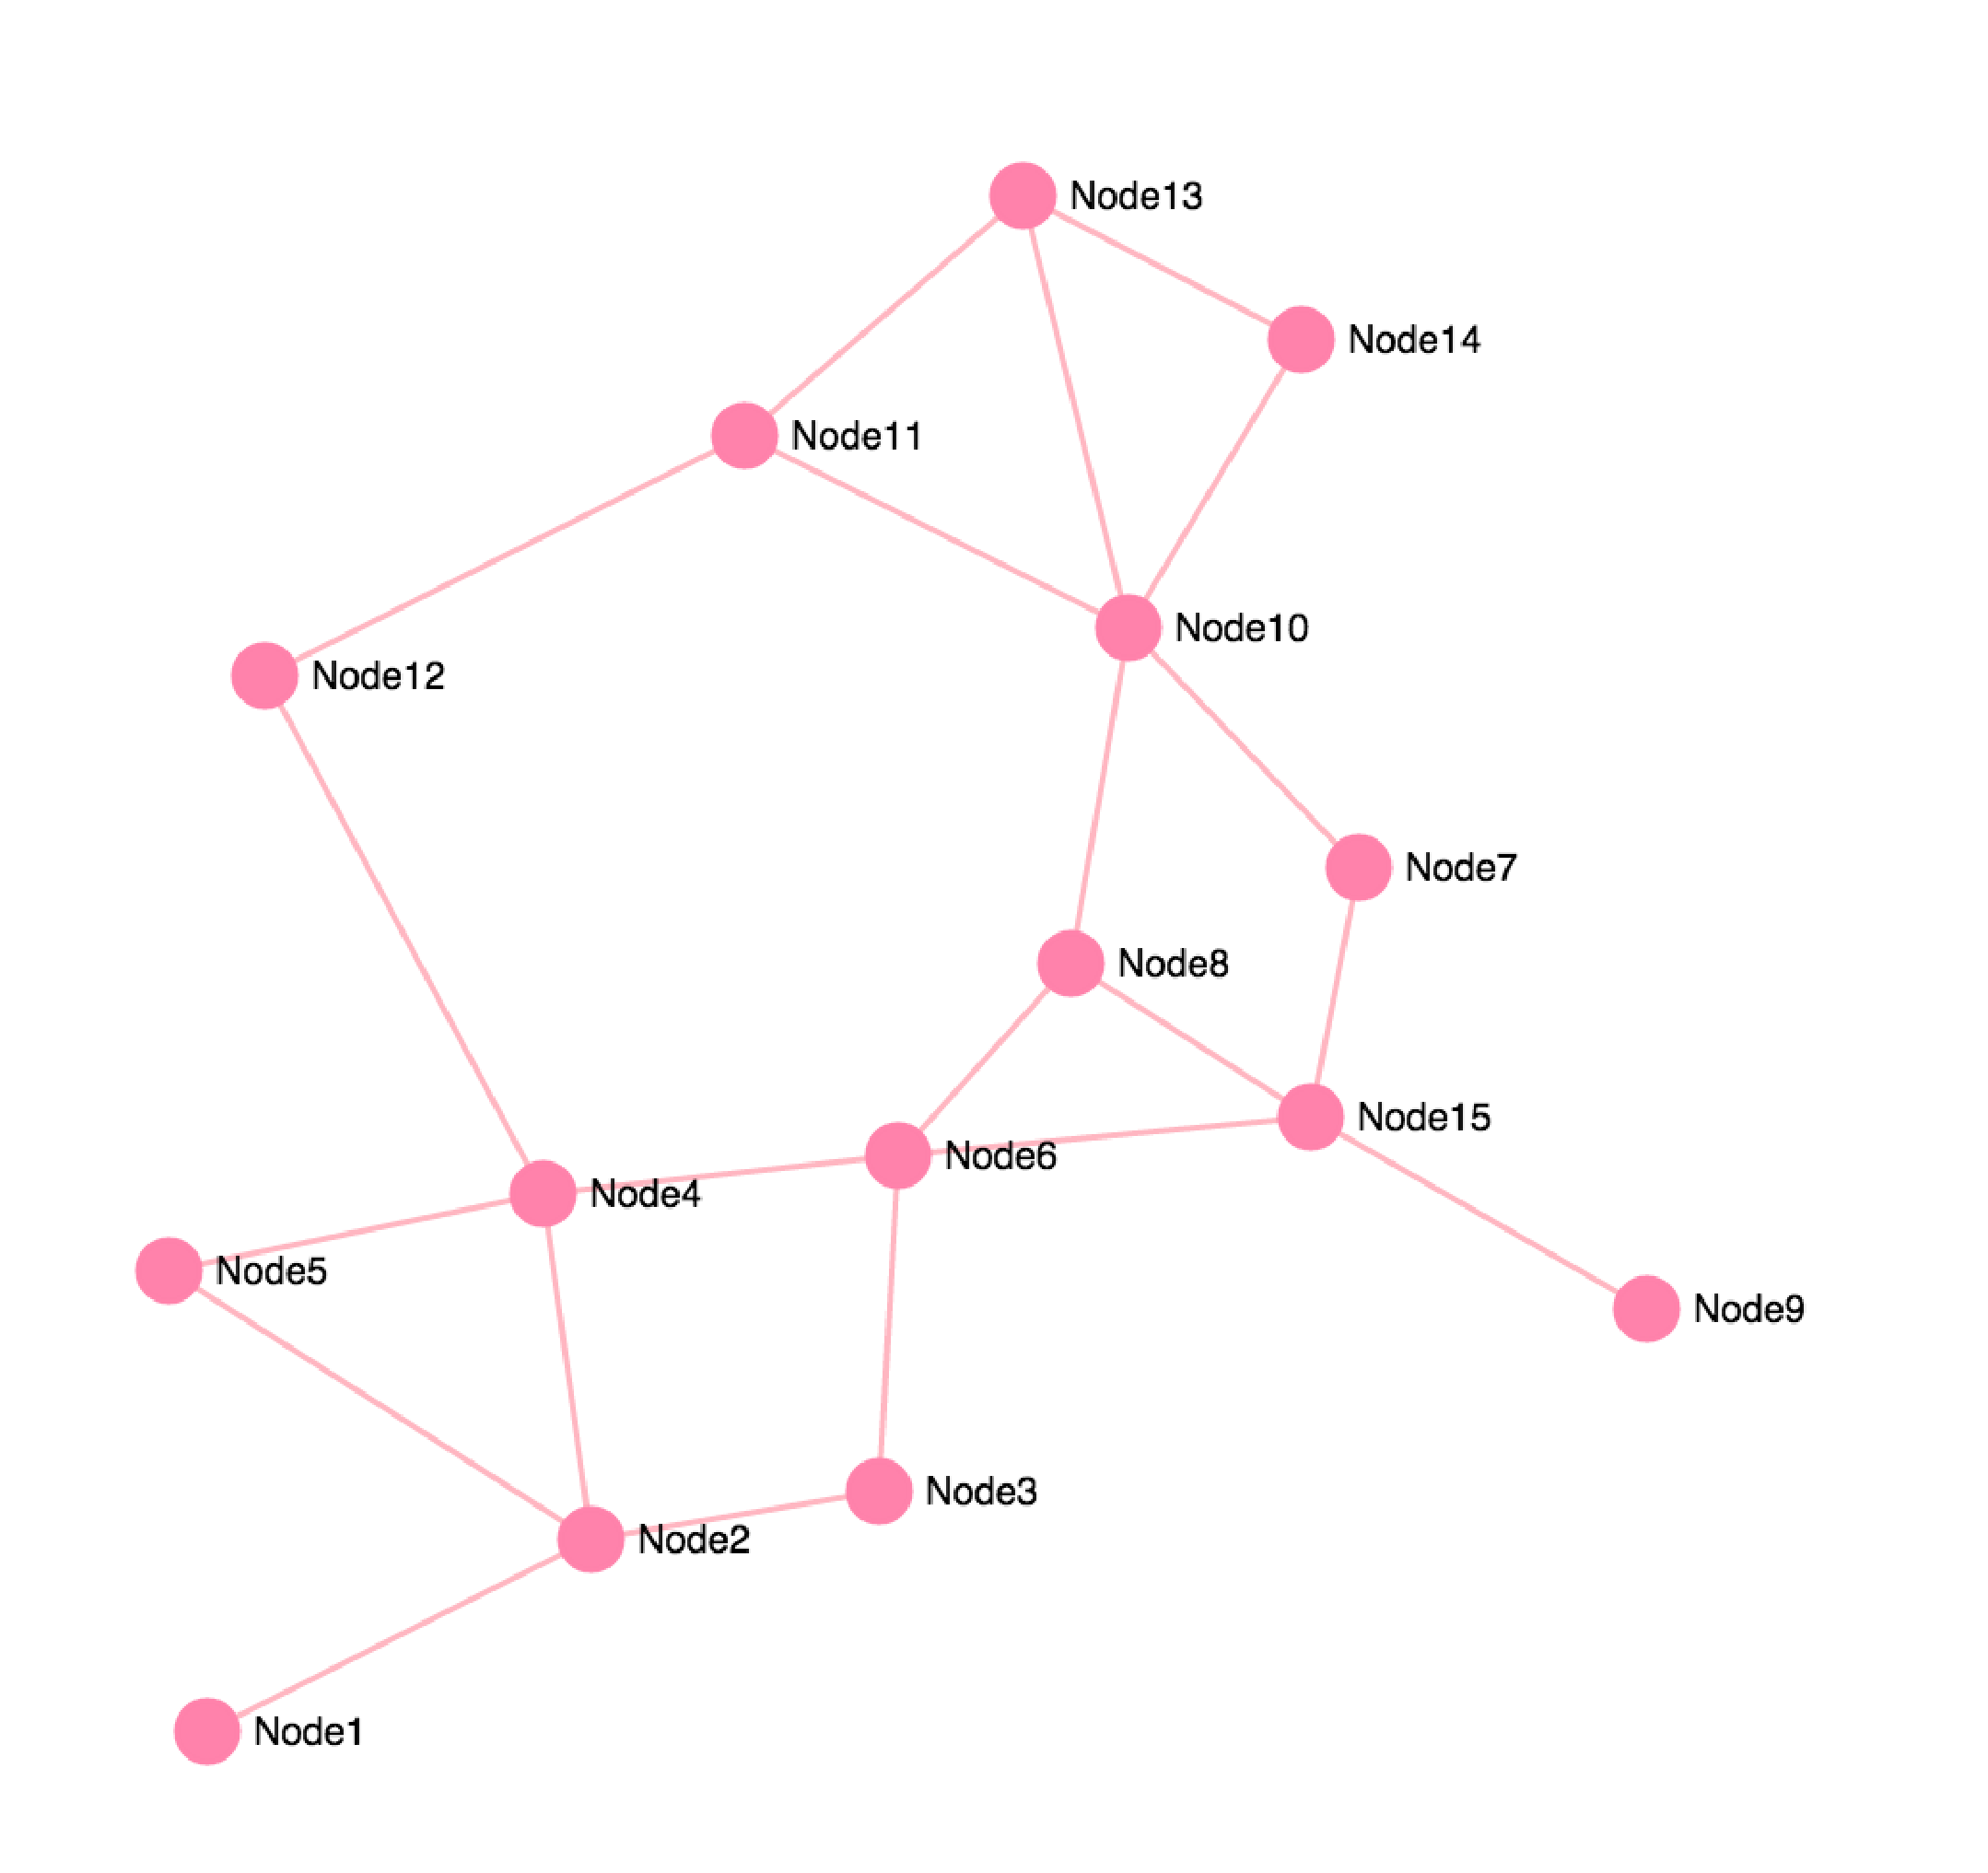
\includegraphics[width=4in]{assets/mandlnetwork_crop.png}
  \end{center}
  \caption{Illustration of Mandl's transit network as a graph}
  \label{fig:MandlNetwork} 
   The transit network including the 15 nodes and 21 edges. The graph is undirected. \emph{\color{red} TODO: Assumptions that it is undirected} Coordinates are correct based on the MandlCoordinates.txt file from \citep{mumford13}
\end{figure}
\section{Performance Criteria}
\label{sec:performanceCriteria}

The criteria used in order to evaluate the performance of the proposed algorithm, which have been adopted by many researchers in the literature \emph{color{red}(Referanser)}.

To measure the efficiency and the quality of our algorithm, the experimental results generated by the proposed algorithm(s) will be compared with the respective results (Mandl, Mumford etc), based on the evaluation criteria in section 3.1.2: 
%These measures were adopted from \citet{kechagiopoulos14}.

\begin{itemize}
\item $d_0 (\%)$ - the percentage of demand satisfied without any transfers, \emph{\color{red}and is calculated as followed:}
\item $d_1 (\%)$ - percentage of total transfer demands where the number of transfers are 1, \emph{\color{red}and is calculated as followed:}
\item $d_2 (\%)$ - percentage of total transfer demands where the number of transfers are 2, \emph{\color{red}and is calculated as followed:}
\item $d_{unsat}$ (\%) - the percentage of demand unsatisfied, which should be equal to zero, \emph{\color{red}and is calculated as followed:}
\item $ATT$  - the average travel times in minutes per transit user (mpu). This incorporates transfer waiting times, \emph{\color{red}and is calculated as followed:}
\end{itemize}


\emph{\color{red} Flyttes til experimental setup, performance comparison? }To demonstrate reliability, we will carry out \emph{\color{red} XX } replicate runs per experiment, recording the average (AVG), best (MAX) and worst (MIN) ant.  
\emph{\color{red} TODO:}

\emph{\color{red} Because of reasons }we believe that ATT and $d_0$ is the most important parameters for determining best and worst, therefore, in the performance comparison experiments, the selection of MAX and MIN will be selected based on these parameters.

\subsection{Selecting MAX Ant}

\begin{algorithm}[H]
$Ant_{i}$ = ant with highest $d_0$\;
$Ant_{j}$ = ant with lowest ATT\;
\eIf{($Ant_{i}$ = $Ant_{j}$)}{
	Select this ant
}
{
	$d_0(\%)$ = $(d_0(lowest) / d_0(highest))*100$\;
	$ATT(\%)$ = $(ATT(lowest) / ATT(highest))*100$\;
	\eIf{ ($ d_0(\%) $ $ \geq $ ATT(\%)) }{
		select $Ant_{j}$
	}
	{
		select $Ant_{i}$
	}
}
 \caption{Selecting MAX Ant}
\end{algorithm}

The comparison is done by calculating the percentage of the difference between the highest and lowest $d_0$ and $ATT$ values. If the difference in the two $d_0$'s is higher than the difference in the two $ATT$'s, the ant with lowest ATT is selected, or else the ant with the highest $d_0$ is selected. As mentioned, a low as possible $ATT$ value and a high as possible $d_0$ value is what we want to achieve.

\subsection{Selecting MIN Ant}
\begin{algorithm}[H]
$Ant_{i}$ = ant with lowest $d_0$\;
$Ant_{j}$ = ant with highest ATT\;
\eIf{($Ant_{i}$ = $Ant_{j}$)}{
	Select this ant
}
{
	$d_0(\%)$ = $(d_0(lowest) / d_0(highest))*100$\;
	$ATT(\%)$ = $(ATT(lowest) / ATT(highest))*100$\;
	\eIf{ ($ d_0(\%) $ $ \leq $ ATT(\%)) }{
		select $Ant_{j}$
	}
	{
		select $Ant_{i}$
	}
}
 \caption{Selecting MIN Ant}
\end{algorithm}
The comparison is also done by calculating the percentage of the difference between the highest and lowest $d_0$ and $ATT$ values. If the difference in the two $ATT$'s is higher than the difference in the two $d_0$'s, the the ant with highest ATT is selected, or else the ant with the lowest $d_0$ is selected. A high $ATT$ and a low $d_0$ is not considered good. 

\section{Experimental Plan}

What experiments or series of experiments are planned. Test the program with many different examples.


\subsection{Plan (endre navn)}
The robustness of our algorithm(s) will be tested. To demonstrate reliability, we will carry out 10 replicate runs per experiment, recording average, max and min.  
%\emph{\color{red} TODO: }

\emph{\color{red} Because of reasons }we believe that ATT and $d_0$ is the most important parameters, therefore the selection of MAX and MIN will be compared to these parameters.

\subsubsection{Selecting MAX Ant}

\begin{algorithm}[H]
$Ant_{i}$ = ant with highest $d_0$\;
$Ant_{j}$ = ant with lowest ATT\;
\eIf{($Ant_{i}$ = $Ant_{j}$)}{
	Select this ant
}
{
	$d_0(\%)$ = $(d_0(lowest) / d_0(highest))*100$\;
	$ATT(\%)$ = $(ATT(lowest) / ATT(highest))*100$\;
	\eIf{ ($ d_0(\%) $ $ \geq $ ATT(\%)) }{
		select $Ant_{j}$
	}
	{
		select $Ant_{i}$
	}
}
 \caption{Selecting MAX Ant}
\end{algorithm}

\emph{\color{red} Kort forklaring }

\subsubsection{Selecting MIN Ant}
\begin{algorithm}[H]
$Ant_{i}$ = ant with lowest $d_0$\;
$Ant_{j}$ = ant with highest ATT\;
\eIf{($Ant_{i}$ = $Ant_{j}$)}{
	Select this ant
}
{
	$d_0(\%)$ = $(d_0(lowest) / d_0(highest))*100$\;
	$ATT(\%)$ = $(ATT(lowest) / ATT(highest))*100$\;
	\eIf{ ($ d_0(\%) $ $ \leq $ ATT(\%)) }{
		select $Ant_{j}$
	}
	{
		select $Ant_{i}$
	}
}
 \caption{Selecting MIN Ant}
\end{algorithm}
\emph{\color{red} Kort forklaring }

\subsection{Stage 1 - Parameter Settings}

In order to study the effect of the variation of the parameters on the objective function values / measures, we conducted a series of experiments to find the most optimal algorithm parameters. The values of these parameters affect directly or indirectly on the final solution quality. The goal is to find some robust parameters which allow the algorithm to find high quality solutions for a wide range of problem instances with different features. 

\subsection{Stage 2 - Performance Comparison}

First we will evaluate results with only the ACO implementation, on Mandl's network and comparing it with the results from other ACO implementations. The aim with this is to test solution quality.

After we have found the optimal algorithm parameters, we will add features from PSO and test the system's performance, comparing it with the respective results. \emph{\color{red}ACO has a known limitation of being stuck on local optima, and the time/space(?) complexity is high.} We will therefore 
add features from PSO - inertial weight, more random in the start and accepting more solutions, knowledge about the best global solution for every iteration, keep the best current solution. After adding SI features from PSO / BSO, we will check whether it is efficient to combine different swarm intelligence methods' attributes to get better results concerning the vehicle routing problem, in order to answer the research question 2 a.

We will test the results comparing it with the performance criteria from section 4.3.

To test whether Neo4J is suited, and if Neo4J Dijkstra's or A* is best concerning run times? The aim is to see if the potential advantages for using a graph database in our implementation, and if this is useful in the optimization process, in order to answer research question 3 and 3 a.


%\begin{enumerate}

%\item Add features from PSO - inertial weight, more random in the start and accepting more solutions, knowledge about the best global solution for every iteration, keep the best current solution.

%\item Evaluate results with only the ACO implementation, on Mandl's network and comparing it with the results from other ACO implementations. The aim with this is to test solution quality and check if we need to change the algorithm / add features from other SI algorithms in order to improve the results, in order to answer research question 2. \emph{\color{red} TODO: Known limitations of ACO. Stuck on local optima, time complexity.}

%\item After adding SI features from PSO / BSO, we will check whether it is efficient to combine different swarm intelligence methods' attributes to get better results concerning the vehicle routing problem, in order to answer the research question 2 a.

%\item And to test whether Neo4J is suited, and if Neo4J Dijkstra's or A* is best concerning run times? The aim is to see if the potential advantages for using a graph database in our implementation, and if this is useful in the optimization process, in order to answer research question 3 and 3 a.

%\end{enumerate}

\subsection{Stage 3 - Time and Space Complexity / Scalability Experiments}

In order to test whether the method is general and not tuned in to run on a single example, we will run the algorithm on other, larger, networks. Mumford included larger networks. Here we will test the time and space complexity.
%The programs are rarely informative if they are designed to run on a single example - Therefore we will test algorithm on other networks, to check whether it is general and not just optimized for Mandl. (Mumford)
Record our run times - test the efficiency of our algorithm.



\section{Experimental Setup}

%The experimental setup should include all data - parameters etc, that would allow a person to repeat your experiments. 
 
\subsection{Parameter Settings}
\label{subsec:parameterSettings_setup}
The parameters tested with different values are described in Table \vref{table:parameters}. Each of these parameters is assigned a default value that will be used when other parameters are tested. The default value of $s$ and $i$ are inspired by the corresponding values described in \citet{salehi-nezhad07}, \citet{poorzahedy11}, \citet{sedighpour14}, and \citet{kechagiopoulos14}. 

$E$, $BR$, $AF$, and $CA$ are parameters unique for the proposed solution, and the default value for these are chosen based on preliminary testing not included in this thesis. 

The default value of $p_b$ is also partly determined based on preliminary testing, but it is also important to acknowledge that the value of $p_b$ is strongly dependent on the value of $p_v$. $p_v$ is, as mentioned in Section \vref{sec:algoInitialization}, the pheromone constant used to determine how much pheromone to be added to all visited edges. Different values of $p_v$ will not be tested because the ants are only concerned about the ratio of the pheromone level on edge $e$ and the summed pheromone level on all the possible edges when choosing which edge to walk. $p_v$ could in fact be any real number, as long as the constant are the same in all cases. $p_v$ is in this thesis sat to 0.1. 

The value of the inertia weight, $IW$, is neither tested with different values partly because the value of $IW$ directly affects $CA$ (as described in Section \vref{sec:algoGeneratingSuperSwarm}) and because implementation of different inertia weight strategies is beyond the scope of this theses. $IW$ is in this thesis sat to 1.0. 

\begin{table}[H]
	\small
	\begin{tabular}{|l|l|l|}
    	\hline
    	Parameters & Description & Default\\
    	\hline
    	$s$ & The SuperSwarm Colony Size & 50\\
    	$i$ & The numbers of iterations (which is the stop criteria) & 50\\
    	$E$ & The percentage of pheromones to evaporate at each iteration & 10\%\\
    	$p_b$ & The pheromone constant added to edges in the best route sets & 0.5\\
    	$BR$ & The percentage of route sets to be granted extra pheromone & 10\%\\
    	$AF$ & The percentage of ants to be followed & 10\%\\
    	$CA$ & The probability that a given ant is declared ``crazy'' & 10\%\\
   	    \hline
    \end{tabular}
    \caption {Parameters to be Tested and their Default Value}.
    \label{table:parameters}
\end{table}

For determining the most fitted parameters, the algorithm will be run 10 time for each candidate value, except for the candidate values of $AF$ and $CA$, which will be run 50 times. $AF$ and $CA$ are directly linked to features from respectively BCO and PSO, and these parameters will therefor be tested more thoroughly.

The parameter values selected will be based on the results concerning the average travel time $ATT$ and the total fitness $TOTFIT$. The selected values will be the ones that produced the lowest average $ATT$ and the lowest $TOTFIT$. The reader recalls from Section \vref{sec:algoEvaluation} that the better the total fitness, the lower the $TOTFIT$ value. If the lowest $ATT$ and the lowest $TOTFIT$ are not achieved by the same parameter value $PV$, the selected value $SV$ is determined by the following formula:

\[
    SV= 
\begin{cases}
    PV_{bestATT},& \text{if } \frac{ATT_{PV_{bestTOTFIT}}}{ATT_{PV_{bestATT}}}\geq \frac{TOTFIT_{PV_{bestATT}}}{TOTFIT_{PV_{bestTOTFIT}}}\\
    PV_{bestTOTFIT},& \text{otherwise}
\end{cases}
\]

Minimum \textit{five} different candidate values are tested for each parameter. The candidate values of $s$ and $i$ are inspired by the corresponding values in the literature described in Section \vref{relatedWork}. The parameters $E$, $BR$, $AF$, and $CA$ are all stated as a percentage and their candidate values will therefor be in the range 0 to 100. $AF$ and $CA$ are the only two tested with 0, because that will help determine the effect of BCO and PSO. As stated above, $p_b$ is dependent on the $p_v$ value, and because $p_v$ is sat to 0.1, $p_b$ will be tested in the range 0.1 to 0.9. The idea of $p_b$ is to ``reward'' the edges in the best route sets, and we have therefor chosen to keep $p_b$ equal to or greater than $p_v$. Further $p_b$ is always lesser than 1.0 to avoid over appreciating the edges in the best route sets, which might result in the ants getting stuck at local optima. 

\subsection{Performance Comparison}

To demonstrate reliability, we will carry out \emph{\color{blue} TODO: XX } replicate runs per experiment, recording the average (AVG), best (MAX) and worst (MIN) ant.  

\emph{\color{blue} TODO: Because of reasons }we believe that ATT and $d_0$ is the most important parameters for determining best and worst ants, therefore, the selection of the MAX and MIN ant will be selected based on these parameters. 

\subsubsection{Selecting MAX ant}
\begin{algorithm}[H]
$Ant_{i}$ = ant with highest $d_0$\;
$Ant_{j}$ = ant with lowest ATT\;
\eIf{($Ant_{i}$ = $Ant_{j}$)}{
	Select this ant
}
{
	$d_0(\%)$ = $(d_0(lowest) / d_0(highest))*100$\;
	$ATT(\%)$ = $(ATT(lowest) / ATT(highest))*100$\;
	\eIf{ ($ d_0(\%) $ $ \geq $ ATT(\%)) }{
		select $Ant_{j}$
	}
	{
		select $Ant_{i}$
	}
}
 \caption{Selecting MAX Ant}
\end{algorithm}


The comparison is done by calculating the percentage of the difference between the highest and lowest $d_0$ and $ATT$ values. If the difference in the two $d_0$'s is higher than the difference in the two $ATT$'s, the ant with lowest ATT is selected, or else the ant with the highest $d_0$ is selected. As mentioned, a low as possible $ATT$ value and a high as possible $d_0$ value is what we want to achieve.

\subsubsection{Selecting MIN ant}
\begin{algorithm}[H]
$Ant_{i}$ = ant with lowest $d_0$\;
$Ant_{j}$ = ant with highest ATT\;
\eIf{($Ant_{i}$ = $Ant_{j}$)}{
	Select this ant
}
{
	$d_0(\%)$ = $(d_0(lowest) / d_0(highest))*100$\;
	$ATT(\%)$ = $(ATT(lowest) / ATT(highest))*100$\;
	\eIf{ ($ d_0(\%) $ $ \leq $ ATT(\%)) }{
		select $Ant_{j}$
	}
	{
		select $Ant_{i}$
	}
}
 \caption{Selecting MIN Ant}

\end{algorithm}

The comparison is also done by calculating the percentage of the difference between the highest and lowest $d_0$ and $ATT$ values. If the difference in the two $ATT$'s is higher than the difference in the two $d_0$'s, the the ant with highest ATT is selected, or else the ant with the lowest $d_0$ is selected. A high $ATT$ and a low $d_0$ is not considered good. 

\subsubsection{Algorithm Parameters}
After running test stage 1, (finding the optimal algorithm parameters), these are the final parameters which will be used in stage 2.

\begin{table}[H]
	\centering
    \begin{tabular}{|l|l|l|l|l|l|l|l|}
 	\hline
 	$s$ & $i$ & $p_{e}$ & $p_{v}$ & $p_{b}$ & $BR$ & $FA$ & $CA$  \\
 	\hline
    ~ & ~ & ~ & ~ & ~ & ~ & ~ & ~ \\
	\hline
    \end{tabular}
    \caption {Final selected parameters}
    Final Parameters from the parameter settings experienced, found in Table \vref{table:parameterSettings2}
    \label{table:finalParameters}
	\end{table}

\subsubsection{Route Set Sizes}
4,6,7 and 8 routes per set.

\subsection{Scalability Experiments}
Time and Space Complexity

\section{Experimental Results}

Results should be clearly displayed and should provide a suitable representation of your results for the points you wish to make. Graphs should be labeled in a legible font and if more than one result is displayed on the same graph then these should be clearly marked.   Please choose carefully rather than presenting every results. Too much information is hard to read and often hides the key information you wish to present. Make use of statistical methods when presenting results, where possible to strengthen the results.  Further, the format of the presentation of results should be chosen based on what issues in the results you wish to highlight. You may wish to present a subset in the experimental section and provide additional results in the appendix.

\subsection{Stage 1 - Parameter Settings}
\label{subsec:parameterSettings_results}

The complete experimental results can be found in Table \ref{table:parameterSettings} in Appendix \ref{appendixC}.

\begin{table}[H]
	\centering
    \begin{tabular}{|l|l|l|l|l|l|l|l|l|}
 	\hline
 	$s$ & $i$ & $p_{e}$ & $p_{v}$ & $p_{b}$ & $BR$  & $IW$ & $FA$ & $CA$  \\
 	\hline
    50 & 50 & 10\% & 0.5 & 0.5 & 10\% & 10\% & 10\%  & 10\%  \\
	\hline
    \end{tabular}
    \caption {Start Values}
    \label{table:parameter_startvalues}
	\end{table}

	\begin{table}[H]
	\centering
    \begin{tabular}{|c|c||c|}
 	\hline
 	Parameters & Candidate values & The best value\\
 	\hline
    $s$ & ~ & ~ \\
    $i$ & ~ & ~ \\
    $p_{e}$ & 1\%, 10\%, 50\%, 90\%, 99\% & 50\% \\
    $p_{v}$ & 0.01, 0.5, 0.9 & ~ \\
    $p_{b}$ & 0.01, 0.5, 0.9 & ~ \\
    $BR$ & ~ & ~ \\
    $IW$ & ~ & ~ \\
    $FA$ & ~ & ~ \\
    $CA$ & ~ & ~ \\
	\hline
    \end{tabular}
    \caption {Parameter settings results}
    \label{table:parameterSettings2}
	\end{table}

\subsection{Stage 2 - Performance Comparison}

\begin{table}[H]
	\centering
    \begin{tabular}{|l|l l l l l l l l|}
    \hline
    Route 1: & ~ & ~ & ~ & ~ & ~ & ~ & ~ & ~ \\
    Route 2: & ~ & ~ & ~ & ~ & ~ & ~ & ~ & ~ \\
    Route 3: & ~ & ~ & ~ & ~ & ~ & ~ & ~ & ~ \\
    Route 4: & ~ & ~ & ~ & ~ & ~ & ~ & ~ & ~ \\
	\hline
    \end{tabular}
    \caption {The best route sets, having four routes, constructed by the proposed algorithm.}
    \label{table:performanceComparison_bestRouteSet4}
	\end{table}

\begin{table}[H]
	\centering
    \begin{tabular}{|l||l|l|l|l|l|}
 	\hline
 	Algorithm & $d_0(\%)$ & $d_1(\%)$ & $d_2(\%)$ & $d_{unsat}(\%)$ & $ATT$ \\
 	\hline
    Mandl[] & ~ & ~ & ~ & ~ & ~ \\
    Nikolic[] & ~ & ~ & ~ & ~ & ~ \\
    Kechapocholous[] & ~ & ~ & ~ & ~ & ~ \\
    Fan and Mumford[] & ~ & ~ & ~ & ~ & ~ \\
   
	\hline
    \end{tabular}
    \caption {Comparing the best route sets, having four routes, constructed by the proposed algorithm with route sets constructed by other approaches.}
    \label{table:performanceComparison_4}
	\end{table}

\subsection{Stage 3 -  Scalability Experiments}
Time and Space Complexity

\chapter{Evaluation and Conclusion}
\label{evaluationAndConclusion}
\section{Evaluation}

When evaluating your results, avoid drawing grand conclusions, beyond that which your results can in fact support. Further, although you may have designed your experiments to answer certain questions, the results may raise other questions in the eyes of the reader. It is important that you study the graphs/tables to look for unusual features/entries and discuss these as well as discussing the main findings in the results. 

\subsection{Parameter Settings}
Remember:
\begin{itemize}
\item $p_v$, $p_b$: giving these values a higher number, results in awarding the local best ants edges by giving them more pheromone, which we observed gave worse results, \emph{\color{red}because get stuck at local optima? blabla}
\item with 100\% crazy ants, the ants did not manage to find a solution \emph{\color{red}because...}. 
\item 0\% crazy ants gave worse results than both 5\% and 10\% CA, where we can conclude that some crazy ants is better than none. But, as we see in the results, more than 10\% CA gives worse results than 0\% CA, so we can conclude that it does not mean the more crazy ants, the better results regarding the final results. But some CA is good for the colony:)
\item Our start values - 10\% on $p_e$, $BR$, $FA$, and $CA$, was actually the best values all along. We could have set these to have worse values in the beginning of the test experiment, and receiving increasing results concerning $TOTFIT$ and $ATT$, but \emph{\color{red} we set the start values to be what we though was best, because???, and with this conclude that our instinct regarding these values was the best.}
\item 100\% and 50\% FA was better than having 0\% following ants; can we conclude that it is better to have following ants, than not have following ants ?
\item Ant colony size ,$s$, parameter testing will be optimized for Mandl network only.
\end{itemize}

\subsection{Neo4j}

Whether Neo4J is suited. Advantages / disadvantages of using a graph database in our implementation (research question 3a)
\section{Discussion}
%Discuss what you managed, and why you had sucess / not success. Show that you understand. In the discussion it is important to include a discussion of not just the merits of the work conducted but also the limitations.
%Svar på research questionsene. %Hva har vi fått til? Hva har vi ikke fått til? Hvorfor fikk vi det til? Hvorfor fikk vi det ikke til? (Små endringer som faktisk kunne blitt gjort, må ikke nevnes, betyr bare at vi har begynt sent på oppgaven.)

Research Question \label{itm:1} has a whole is answered in Chapter \label{relatedWork}.

\textbf{Goal:}
\begin{itemize}
\item  Increase the number of public transportation passengers by making urban transit networks more efficient.
\end{itemize}

\textbf{Research Questions:}
\begin{enumerate}[label=\textbf{\arabic*})]
\item[\textbf{2)}]
    \begin{enumerate}

    \item[(a)]  \textbf{Is it efficient to add attributes from other swarm intelligence-methods in order to improve the ant colony optimization algorithm?}

    * Based on results, we see that is efficient to add attributes from other SI methods. 

    * ACO has previously shown that it manage to find good solutions - [ref]. It manage to find good solutions fast, by following pheromone trails. The disadvantage is that pheromone trails laid can be a local optima.
    
    * As seen in the ACO vs SSO performance comparison one can see that SSO performs overall better than a plain ACO implementation. But as mentioned in the evaluation. ACO does not possess the memory feature. Which enables the ants to remember which node it has visited within the same route set. This feature makes it possible for the ants to create more route sets that are connected, this is important, because a passenger should be able to travel from every node to every other node withing the route network. This results in a lot of ACOs route sets will be discarded, and therefore not taken into evaluation. This means ACO will have less good route sets to be evaluated, and therefore increases the chance of finding the optimal route set. 

    * However. As we observed in the parameter settings experiments. When adding the additional parameters from other swarm inspired methods. These both increased the performance of the algorithm. 

    * The feature added from PSO - where the particles explore more in the early iterations and become more organized in the later iterations. The PSO algorithms have shown to find good solutions[ref], because they manage to get out of a local optima. This feature was added to the proposed. And we observed that adding this additional feature to ACO managed to increase the performance of our algorithm. This feature enables the algorithm to explore new (possible better) routes, regardless of the pheromone value laid on the edges.
    %global best solution of all iterations

    * In BCO - communicate and share knowledge. The once who have found good routes, share this knowledge with other bees, and make more bees will follow the same path. BCO has proven too find good solutions[ref], and this reflects the implementation of this feature in the proposed algorithm. Wee see that rewarding the very best routes with a high amount of pheromone is beneficial for the performance of the algorithm. 

    \item[(b)]  \textbf{How does the proposed method perform compared to methods published in literature?}
    * As stated in Evaluation, the proposed algorithm produce the best average travel time, compared to all the published literature this algorithm is compared to. It performs best concerning the average travel time, regardless of the route set size, on the Mandl network. 
    * The rest of the performance criteria, concerning the number of transfers - the algorithm performs just below average compared to the other approaches. 
    * Again, is it worth mentioning that a direct route is still an important factor when selecting the best route set. But, this approach sat to favor a small average travel time.
    * This is because. 
    * Whether a passenger would travel a little longer and travel direct, versus changing a route once and decrease the travel time is a matter of preferences. And as one can see, you have to choose one at the expense of the other. But, as mentioned in the motivation, citizens often prefer private transportation because of the decreased travel time. 

    \item[(c)]  \textbf{Is it possible to apply the proposed algorithm to optimize urban transit routes in real urban cities?}


    \end{enumerate}
\item[\textbf{3)}]
	\begin{enumerate}
	\item[(b)]  What are the potential advantages and disadvantages of using a graph database in our implementation?
    \end{enumerate}
\end{enumerate}

\textbf{\color{blue} Til diskusjon:}

The parameters tested and used are specifically tuned for Mandl's Transit Network containing 4 routes, with maximum 8 nodes in one route, but the same parameters are used when testing with 6, 7, and 8 routes as well. This may be considered a weakness, because metaherustic methods, such as the one proposed in this thesis, requires calibration of parameters with respect to the problem at hand \citep{dobslaw09}.

The proposed method requires input on a particular form. Both nodes and their coordinates, travel time between nodes and the demand between nodes needs to be provided on a particular form in an .txt-document. This may be considered as a weakness of the method, but implementing support for retrieving the mentioned data on another form are considered as fairly easy.


\section{Contributions}

%What are the main contributions made to the field and how significant are these contribution.

%

In this thesis, we proposed a system for the urban transit routing problem. The proposed Combined Swarm System creates optimal urban transit routes on Mandl's network\citep{mandl79}, and shows especially promising results concerning the average travel time per transit user. We have demonstrated that the performance of a generic ant colony optimization algorithm improves when adding additional attributes inspired by other swarm intelligence-methods. %siste setning på omformuleres


%The system developed is based on  Swarm Intelligence methods. We showed that adding additional attributes to a classic Ant colony optimization method clearly[hardt å melde?] improved the performance. The proposed SuperSwarm optimization system 

\section{Future Work}

Consider where you would like to extend this work. These extensions might either be continuing the ongoing direction or taking a side direction that became obvious during the work. Further, possible solutions to limitations in the work conducted, highlighted in Discussion may be presented.

Future work?: Travel demand can be estimated by examining ticket sales, carrying out a survey, or undertaking analysis. This is difficult in practice, because demand is dynamical and highly sensitive to factors such as pricing and quality of service. In addition to satisfying customer demand, design guidelines are determined by many additional factors, including the street environment and management policies by the local government\citep{fan09}.

One of the main handicaps of urban transportation systems is estimating is rather expensive and therefore not not frequently.In reality the demand is different each time of day and to deal with this problem average demand has to be used or the max demand. It is no use finding optimal sets of lines for different hours of the day, because the organization problems would become enormous and also no passenger would be interested in having different lines at different times. In addition to varying travel and waiting times, also change during the day. The transportation times should then include the average transportation times. \citep{mandl79}

Traffic assignment includes finding the number of people traveling along a specific edge. 
To know how many will use a certain edge. Total flow between each pair of nodes is called the traffic assignment problem.
%and supplies the planner of a road network with important information about the flow density. Kleins alg for minimum cost flow)
%It is vital to minimizing changes and some behavior according to a weighted sum of transportation and waiting time. The flow of each edge it computes as the sum of all people using the edge by one of the two paths. The flow on each arc of each line is not completely defined, because if more than one line proceeds along the same arcs, people might use both of them along these arcs, thus the flow assignment to lines is not unique. 





\cleardoublepage

\bibliographystyle{apalike}
\bibliography{bibl}


\clearpage

\begin{appendices}
\chapter{Protocol}
\label{appendixA}

%TODO: The final protocol with the final search term and justifications.
%Ref: https://raw.githubusercontent.com/kenborge/slr-scbw/master/sections/protocol.tex
\noindent
\begin{table}[h]
\resizebox{12.5cm}{!} {

    \hspace*{-2.25cm}
    \begin{tabular}[c]{| m{1.25cm} | m{1.5cm} | m{1.8cm} | m{1.5cm} | m{1.5cm} | m{1.5cm} | m{1.3cm} | m{1.5cm} | m{1.5cm} |}
    \hline
    & \textbf{Group 1} & \textbf{Group 2} & \textbf{Group 3} & \textbf{Group 4} & \textbf{Group 5} & \textbf{Group 6} & \textbf{Group 7} & \textbf{Group 8} \\ \hline   
    \textbf{Term1} & Train & Path optimization & Bee colony optimization & Transit & Artificial intelligence & Multi agent & Routing & Neo4j \\ \hline
    \textbf{Term2} & Plane & \hspace{0pt}Scheduling optimization & Particle swarm optimization & \hspace{0pt}Transportation & AI & & & Graph database \\ \hline
    \textbf{Term3} & Bus & Route optimization & Swarm intelligence & Traffic & Machine Learning & & & \\ \hline
    \textbf{Term4} & Delivery & Planning & Ant colony optimization & Vehicle & & & & \\ \hline
    \textbf{Term5} & & Multimodal & BCO & & & & & \\ \hline
    \textbf{Term6} & & & PSO & & & & & \\ \hline
    \textbf{Term7} & & & ACO & & & & & \\ \hline
    \end{tabular}\hspace*{-2.25cm}
    
    }
    \caption{Matrix of search terms}
    \label{table:searchterms}
\end{table}

\section{Search Terms}

\begin{itemize}

\item Group 1: Train, plane, bus, delivery
\item Group 2: Path optimization, Scheduling Optimization, Route Optimization, Planning, Multimodal
\item Group 3: Bee colony optimization, Particle swarm optimization, Swarm intelligence, Ant colony optimization, BCO, PSO, ACO
\item Group 4: Transit, Transportation, Traffic, Vehicle
\item Group 5: Artificial Intelligence, ai, Machine Learning
\item Group 6: Multi-agent
\item Group 7: Routing
\item Group 8: Neo4j, Graph database

\end{itemize}

\section{Complete Search Term}
\label{searchterm}

\textit{(train OR plane OR bus OR delivery) AND (``path optimization'' OR ``scheduling optimization'' OR ``route optimization'' OR planning OR multimodal) AND (``bee colony optimization'' OR ``particle swarm optimization'' OR ``swarm intelligence'' OR ``ant colony optimization'' OR bco OR pso OR aco) AND (transit OR transportation OR traffic OR vehicle) AND (``artificial intelligence'' OR ai OR ``machine learning'') AND ``multi-agent'' AND routing)}

% Har ditcha gruppe 8 i den "komplette søketermen", fordi vi ikke bruker gruppe 8 som en del av literatursøket, men kun til å "prove a point"

 %Lol & Group 1 & Group 2 & Group 3 & Group 4 & Group 5 & Group 6 & Group 7 & Group 8 \\ \hline
 %   Term 1 & Train & Path optimization & Bee colony optimization & Transit & Artificial intelligence & Multi agent & Routing & Neo4j \\ \hline


\section{Research Questions}
To conduct a structured literature review it is vital to decide the problem to be solved, referred to as P, and the constraints used to guide the search, referred to as C.
\newline
\newline
One of the goals for the environment package for transportation in Trondheim, ``Miljøpakken'', is to reduce percentage of people travelling with cars from 58 \% to 50 \% by 2018 \citep{website:miljopakken}. If this goal is reached, it will be an increased need for public transportation in Trondheim. There has never been done any optimization of the bus routes in Trondheim, the existing solution is purely based on experience. The problem formulation for this thesis was therefore based on the idea to improve todays solution by optimizing the bus routes using AI-methods. (And as a result of this satisfy the same amount of users today with less resources.)

\begin{itemize}
\item \textbf{P:} “Optimizing the bus routes in Trondheim using AI-methods. “ This problem can be characterized as a \textit{General Pickup and Delivery Problem (GPDP)} \citep[p.22-25]{vehiclerouting}.  
\item \textbf{C:} 
    \begin{enumerate}
        \item To optimize the bus routes in Trondheim we wanted to explore the possibility using methods from swarm intelligence. This idea came from an initial, non-structured literature review were we did a broad search among different artificial intelligence methods and route optimizing. %Todo: Kanskje skrive litt mer om dette? Evt. sitere noe literatureshit
        \item We believe that a part of solving the problem, P, is how we choose to represent the network of the bus routes in Trondheim. The chosen algorithms to optimize the routes with respect to minimize the number of resources used will use this representation. We have some experience with the graph database Neo4j. Neo4j has several benefits that we believe we can take advantage of when solving P, including a natural node-edge-structure and the possibility of saving information to both the nodes and edges. We envision that the nodes will represent bus stops, and the edges will represent the connectivity between the stops. 
    \end{enumerate}
\end{itemize}

\textbf{This gives us the following research questions:}
%\begin{enumerate}
%\item What are the existing solutions to this problem?
%\item Which swarm intelligence methods is best suited for optimizing? 
%\item Is it practicle to represent and work with this route network as a graph database for this kind of methods?
%\item Does this solution help optimize the bus routes? 
%\end{enumerate}

\begin{enumerate}[label=\textbf{\arabic*})]
\item 
    \begin{enumerate}
    \item Is swarm intelligence methods suitable for the vehicle routing problem?
    \item What is the state-of-the-art in solving vehicle routing problems using swarm intelligence methods?
    \item What changes have been done to the classical swarm intelligence-methods to improve them?
    \item Have there been any attempts to combine different swarm intelligence-methods?
    \end{enumerate}
\item
    \begin{enumerate}
    \item Is it efficient to combine attributes from different swarm intelligence-methods to solve the vehicle routing problem?
    \item Is it possible to apply our algorithm to optimize bus routes in urban cities?
    \end{enumerate}

\item
    \begin{enumerate}
    \item What are the potential advantages and disadvantages of using a graph database in our implementation?
    \item Is the features of graph databases useful in the optimization process? 
    \end{enumerate}
\end{enumerate}

%Todo: Skrive om Zotero

\section{Inclusion Criteria}
To exclude irrelevant literature, some inclusion criterias were decided to ensure a level of relevance to the very first pool. First of all, duplicate literature, book of chapters, book of abstracts, book of references, literature not written in english, books, and literature with cleary irrelevant titles (for example literature from different research areas) were removed based on title. After that, we decided to filter out relevant literature based on the abstracts. Because we had relatively many sources to related literature after the initial filtering (367), we decided that we wanted the abstracts (or the keyword section) to explicitly mention swarm intelligence or algorithms associated with swarm intelligence, while it also described a problem connected to vehicle routing. For our literature review we decided to use the inclusion criterias solely on the title, abstract and keywords. After a discussion and reading a few abstracts we landed on the following inclusion criterias:
\begin{itemize}
\item The main concern is route optimization focusing on vehicles. 
\item The study focuses on the use of swarm intelligence.
\item The literature must contain an abstract. 
\item The literature must still excist (some literature were removed from its original source).
\item The literature must be free of charge.
\end{itemize}

After the inclusion criteria filtering, we had 42 sources to related literature, including scientific papers and master theses. 

\section{Quality Criteria} 

\begin{enumerate}
\item How relevant is it?
\begin{enumerate}
\item Is the problem of the research a vehicle routing problem?
\item Is swarm intelligence the main optimization method? 
\end{enumerate}
\item Is there is a clear statement of the aim of the research?
\item Is the study put into context of other studies and research?
\item Are system of algoritmic design decisions justified?
\item Is the test data set reproducible?
\item Is the study algorithm reproducible?
\item Is the experimental procedure thoroughly explained and reproducible?
\item Is it cleary stated in the study which other algorithms the study`s algorithm(s) have been compared with?
\item Are the performance metrics used in the study explained and justified?
\item Are the test results thorougly analysed?
\item Does the test evidence support the findings presented?
\item Has the architecture been implemented (and published)?
\item Is the amount/quality of citation satisfactory? ($<$ $\frac{1}{3}$  self-citation and $>$ 10 citations)
\end{enumerate}

\subsection{Scoring}
Point 1-13 was given a score, with the granularity of 0 (no), $\frac{1}{2}$ (partly), and 1 (yes). For this structured literature review we wanted to emphasize on the quality criteria that covered the relevance. We read some literature that were quite good regarding to the example structure and composition, but not relevant for our thesis. Therefore, we chose to multiply the 1a and 1b quality criteria with 3. Table \ref{table:literature} shows the papers that were read and scored according to the quality criteria: 

\begin{table}[H]
    {
    \tiny
    \hspace*{-2cm}
    \resizebox{16.5cm}{!} {
    \begin{tabular}[c]{|m{6.5cm}|c|c|c|c|c|c|c|c|c|c|c|c|c|c|c|}
        \hline
        \textbf{Title} & \textbf{1a} & \textbf{1b} & \textbf{2} & \textbf{3} & \textbf{4} & \textbf{5} & \textbf{6} & \textbf{7} & \textbf{8} & \textbf{9} & \textbf{10} & \textbf{11} & \textbf{12} & \textbf{13} & \textbf{Total} \\ \hline
        \textit{``A comprehensive review of firefly algorithms''}&0&3&1&1&1&0&1&0&1&0.5&0&0&0&1&9 \\ \hline
        \textit{``Adaptive Comprehensive Learning Bacterial Foraging Optimization and Its Application on Vehicle Routing Problem with Time Windows''}&1.5&1.5&0.5&1&0.5&1&1&1&1&1&1&0&0&1&12 \\ \hline
        \textit{``Adapt-Traf: An adaptive multiagent road traffic management system based on hybrid ant-hierarchical fuzzy model''}&1.5&1.5&1&1&1&0.5&0.5&1&0&1&1&1&0&1&12 \\ \hline
        \textit{``A Design of Intelligent and Autonomous Public Transportation System by Co-evolution''}&3&1.5&0&0&0.5&0&0&0&0&0&0&0&0&0.5&5.5 \\ \hline
        \textit{``A fast solution method for the time-dependent orienteering problem''}&3&1.5&1&1&0.5&1&1&1&1&1&1&1&0&1&15  \\ \hline
        \textit{``Agent-based Simulation for UAV Swarm Mission Planning and Execution''}&0&1.5&1&1&0.5&0.5&1&0.5&1&0.5&0.5&0.5&0&1&9.5 \\ \hline
        \textit{``A hybrid particle swarm optimization approach for the sequential ordering problem''}&1.5&3&1&1&1&1&1&1&1&1&0.5&0.5&0&0.5&14 \\ \hline
        \textit{``An ant based algorithm approach to vehicle navigation''}&3&3&1&0.5&1&0.5&1&1&0.5&1&1&0.5&0&0.5&14.5 \\ \hline
        \textit{``An Ant Based Simulation Optimization for Vehicle Routing Problem with Stochastic Demands''}&1.5&3&1&1&1&1&1&1&1&0.5&1&0.5&0&1&14.5 \\ \hline
        \textit{``An Ant Colony Optimization Approach to Solve Cooperative Transportation Planning Problems''}&1.5&1.5&0&1&0.5&0.5&1&1&1&1&1&1&0&1&12 \\ \hline
        \textit{``An Ant System application to the Bus Network Design Problem: an algorithm and a case study''}&3&3&1&1&1&1&1&1&1&1&1&1&0&1&17 \\ \hline
        \textit{``An exploration of the literature on the use of 'swarm intelligence-based techniques' for public service problems''}&1.5&3&1&0.5&1&1&0.5&1&0.5&1&0.5&0.5&0&1&13 \\ \hline
        textit{``An improved Ant Colony algorithm for Urban Transit Network Optimization''}&3&3&1&1&1&1&1&1&1&1&1&1&0&1&17 \\ \hline
        \textit{``An Inverted Ant Colony Optimization approach to traffic''}&1.5&3&1&1&1&1&1&1&0.5&1&1&0.5&0&1&14.5 \\ \hline
        \textit{``Ant Colony Optimization''} &1.5&3&0.5&0.5&0.5&1&0.5&0.5&0.5&0.5&0&0&0&0&9 \\ \hline
        \textit{``Ant colony optimization for best path planning''}&3&3&1&1&1&1&1&1&0.5&1&1&1&0&0.5&16 \\ \hline
        \textit{``Ant colony optimization techniques for the vehicle routing problem''}&3&3&1&0&0.5&0.5&0.5&0.5&1&1&1&1&0&1&14 \\ \hline
        \textit{``Ant dispersion routing for traffic optimization''}&1.5&1.5&1&1&1&1&1&1&1&1&1&0.5&0&1&13.5 \\ \hline
        \textit{``A parallel ant colony algorithm for bus network optimization''}&3&3&1&1&0.5&1&1&1&0.5&1&1&1&0&1&16 \\ \hline
        \textit{``A review of ant algorithms''}&1.5&3&0.5&1&0.5&1&1&1&1&1&1&0.5&0&1&14 \\ \hline
        \textit{``A simultaneous transit network design and frequency setting: Computing with bees''} &3&3&1&1&1&1&1&1&1&1&1&1&0&1&17 \\ \hline
        \textit{``A Study on Bus Routing Problem: An Ant Colony Optimization Algorithm Approach''} &3&3&1&1&1&0.5&0.5&0.5&1&0.5&0.5&0.5&0&0&13 \\ \hline
        \textit{``A Swarm Based Method for Solving Transit Network Design Problem''}&3&3&0.5&1&0.5&0.5&1&1&1&1&0.5&0.5&0&0.5&14 \\ \hline
        \textit{``Bi-objective bimodal urban road network design using hybrid metaheuristics''}&1.5&1.5&1&1&0.5&1&1&1&1&1&1&1&0&1&13.5 \\ \hline
        \textit{``Bus Transit Service Optimization–The State-of-the-Art. State-of-the-Practice, and Challenges''}&1.5&0&1&0&1&1&0.5&0.5&0.5&0.5&0.5&0.5&0&0.5&8 \\ \hline
        \textit{``Combining new Fast Opposite Gradient Search with Ant Colony Optimization for solving travelling salesman problem''}&0&3&1&1&0.5&1&1&1&1&1&1&0.5&0&1&13 \\ \hline
        \textit{``Computing with bees: Attacking complex transportation engineering problems''}&1.5&3&1&1&1&1&1&1&0&1&1&1&0.5&1&15 \\ \hline
        \textit{``Data mining with various optimization methods''}&0&1.5&1&1&0.5&0&1&0.5&1&1&1&1&0.5&1&11 \\ \hline
        \textit{``Designing a multimodal feeder network by covering stops with different modes''}&1.5&3&1&1&1&0&0.5&1&0&1&1&1&0.5&1&13.5 \\ \hline
        \textit{``Dynamic Fuzzy Logic-Ant Colony System-Based Route Selection System''}&3&3&0.5&1&1&0.5&0.5&0.5&1&1&1&1&0.5&1&15.5 \\ \hline
        \textit{``Multimodal Feeder Network Design Problem: Ant Colony Optimization Approach''}&1.5&3&1&1&0.5&0&1&0.5&0&1&1&1&0.5&1&13 \\ \hline
        \textit{``Optimization of a Transit Services Model with a Feeder Bus and Rail System Using Metaheuristic Algorithms''}&3&1.5&0.5&1&1&0&1&0.5&1&1&1&1&0.5&1&14 \\ \hline
        \textit{``Optimization of Large Transport Networks Using Ant Colony Heuristic''}&0&3&0.5&0.5&0.5&0.5&1&0.5&0&1&0.5&1&0.5&1&10.5 \\ \hline
        \textit{``Optimizing bus transit network with parallel ant colony algorithm''}&1.5&3&1&0.5&0.5&1&1&0&1&1&1&1&0.5&1&14 \\ \hline
        \textit{``Real-time route planning of the public transportation system''}&3&3&1&0&0.5&0.5&1&0.5&0.5&1&0.5&1&0.5&1&14 \\ \hline
        \textit{``Route Optimization for Bus Dispatching Based on Improved Ant Colony Algorithm''} &3&3&0.5&0&0.5&0.5&1&0.5&0&0&0.5&1&0.5&0.5&11.5 \\ \hline
        \textit{``Solving the open vehicle routing problem by a hybrid ant colony optimization''}&3&3&1&1&1&1&1&1&1&1&1&1&0.5&1&17.5 \\ \hline
        \textit{``Solving the Urban Transit Routing Problem using a particle swarm optimization based algorithm''}&3&3&1&1&1&1&1&1&1&1&1&1&0.5&1&17.5 \\ \hline
        \textit{``The Application of Artificial Intelligence Hybrid in Traffic Flow''}&0&3&0.5&0&0&0&0&0&0&0&0&0&0&1&4.5 \\ \hline
        \textit{``Transit network design by Bee Colony Optimization''}&1.5&3&1&1&1&1&1&1&0.5&0&0.5&1&0.5&1&14 \\ \hline
        \textit{``Transportation Modeling: An Artificial Life Approach''} &1.5&3&1&0.5&0.5&0&0.5&0.5&0.5&0.5&0.5&1&0.5&1&11.5 \\ \hline
        \textit{``Transport Modeling by Multi-Agent Systems: A Swarm Intelligence Approach''}&3&3&0.5&0.5&0.5&0&0&0&0.5&0&0&0&0&1&9 \\ \hline

    \end{tabular}
    } 
    }
\caption{Quality Criteria Scoring}\label{table:literature}
\end{table}\hspace*{-2cm}

\section{Selecting the final literature}
When selecting the final literature we decided to do this solely based on the quality criteria scores. The average score of the read literature was 13.01 $\approx$ 13. We decided that literature given a score $\geq{1.5}$ above average were selected. After this sorting we ended up with 14 final literature. These 12 literature are going to create the foundation of our thesis. Table \ref{table:finalliterature} shows the selected literature. 

\begin{table}[!htb]
    {
    \begin{center}
    \small
    \begin{tabular}[c]{| m{6cm} | m{6cm} |}
        \hline
        \textbf{Title} & \textbf{Author} \\ \hline
        \textit{``An ant based algorithm approach to vehicle navigation''} & Salehi-nezhad and Farrahi-Moghaddam \\ \hline
        \textit{``An Ant Based Simulation Optimization for Vehicle Routing Problem with Stochastic Demands''} & Tripathi et al. \\ \hline
        \textit{``An Ant System application to the Bus Network Design Problem: an algorithm and a case study ''} & Poorzahedy and Safari \\ \hline
        \textit{``An improved Ant Colony algorithm for Urban Transit Network Optimization''} & Jiang et al. \\ \hline
        \textit{``An Inverted Ant Colony Optimization approach to traffic''} & Dias et al. \\ \hline
        \textit{``Ant colony optimization for best path planning''} & Hsiao et al. \\ \hline
        \textit{``A parallel ant colony algorithm for bus network optimization''} & Yang et al. \\ \hline
        \textit{``A simultaneous transit network design and frequency setting: Computing with bees''} & Nikolić and Teodorović \\ \hline
        \textit{``Computing with bees: Attacking complex transportation engineering problems''} & Panta and Du San Teodorovi \\ \hline
        \textit{``Dynamic Fuzzy Logic-Ant Colony System-Based Route Selection System''} & Salehinejad and Talebi \\ \hline
        \textit{``Solving the open vehicle routing problem by a hybrid ant colony optimization''} & Sedighpour et al. \\ \hline
        \textit{``Solving the Urban Transit Routing Problem using a particle swarm optimization based algorithm''} & Kechagiopoulos and Beligiannis \\ 
        \hline
    \end{tabular}
    \end{center}
    } 
\caption{Final literature}\label{table:finalliterature}
\end{table}
\section{Search Engines and Search Strings}
\label{sec:searchEngines}
%TODO: Write about the different what kind of results the different search engines gave with differet search terms. (With and without graph database)
%Ref: https://raw.githubusercontent.com/sandsmark/slr-scbw/master/subsections/search_engines.tex
In this structured literature review, we decided to search in seven different search engines. The process of deciding which search engines to use was strongly influenced by the suggestions in \citep{kofod2014}. The complete search term, described in Section \vref{searchterm}, is built on terms from seven different groups. In addition to the search of the complete search, a search consisting of one additional group (group 8) was conducted in each of the different search engines. Group 8 consists of the words ``neo4j'' and ``graph database''. This additional search was done to investigate if the combination of swarm technology and graph databases to solve a route optimization problem already had been studied. The results from our search show that our search term combined with ``neo4j'' or ``graph database'' gave zero findings.  


\subsection{ACM Digital Library}
\textbf{Notes:} ACM Digital Library did not support a mix of ANDs and ORs in its initial input field, but this was possible in advanced search. The search string was not modified, and the first search gave a satisfactory number of results. 
\newline
\newline
\textbf{Queries:}
\begin{itemize}
\item (Train OR plane OR bus OR delivery) AND (``path optimization'' OR ``scheduling optimization'' OR ``route optimization'' OR planning OR multimodal) AND (``bee colony optimization'' OR ``particle swarm optimization'' OR ``swarm intelligence'' OR ``ant colony optimization'' OR bco OR pso OR aco) AND (transit OR transportation OR traffic OR vehicle) AND (``artificial intelligence'' OR ai OR ``machine learning'') AND ``multi agent'' AND routing
\end{itemize}
\par \textbf{Date of search:} 2014-11-10 
\par \textbf{Results:} 19
\begin{itemize}
\item (Train OR plane OR bus OR delivery) AND (``path optimization'' OR ``scheduling optimization'' OR ``route optimization'' OR planning OR multimodal) AND (``bee colony optimization'' OR ``particle swarm optimization'' OR ``swarm intelligence'' OR ``ant colony optimization'' OR bco OR pso OR aco) AND (transit OR transportation OR traffic OR vehicle) AND (``artificial intelligence'' OR ai OR ``machine learning'') AND ``multi agent'' AND routing AND (``graph database'' OR neo4j)
\end{itemize}
\par \textbf{Date of search:} 2014-11-10 
\par \textbf{Results:} 0


\subsection{ScienceDirect}
\textbf{Notes:} In ScienceDirects advanced search it was only possible to perform a full text search. The first search was within ``all sciences'' and this retrieved 100 results. The next search was therefore just within ``Computer Science'', which gave less, but a lot more relevant literature. In addition to this books were excluded from the results.
\newline
\newline
\textbf{Queries:}
\begin{itemize}
\item (Train OR plane OR bus OR delivery) AND (``path optimization'' OR ``scheduling optimization'' OR ``route optimization'' OR planning OR multimodal) AND (``bee colony optimization'' OR ``particle swarm optimization'' OR ``swarm intelligence'' OR ``ant colony optimization'' OR bco OR pso OR aco) AND (transit OR transportation OR traffic OR vehicle) AND (``artificial intelligence'' OR ai OR ``machine learning'') AND ``multi agent'' AND routing
\end{itemize}
\par \textbf{Date of search:} 2014-11-10 
\par \textbf{Results:} 60
\begin{itemize}
\item (Train OR plane OR bus OR delivery) AND (``path optimization'' OR ``scheduling optimization'' OR ``route optimization'' OR planning OR multimodal) AND (``bee colony optimization'' OR ``particle swarm optimization'' OR ``swarm intelligence'' OR ``ant colony optimization'' OR bco OR pso OR aco) AND (transit OR transportation OR traffic OR vehicle) AND (``artificial intelligence'' OR ai OR ``machine learning'') AND ``multi agent'' AND routing AND (``graph database'' OR neo4j)
\end{itemize}
\par \textbf{Date of search:} 2014-11-10 
\par \textbf{Results:} 0


\subsection{CiteSeer}
\textbf{Notes:} In CiteSeer you cannot perform a search within title, abstract and keywords at the same time. It was therefore conducted a full text search by adding the element text:() to the query.  Some of the retrieved literature had an unknown title with unknown authors, so theese were excluded from the results. 
\newline
\newline
\textbf{Queries:}
\begin{itemize}
\item text:((Train OR plane OR bus OR delivery) AND (``path optimization'' OR ``scheduling optimization'' OR ``route optimization'' OR planning OR multimodal) AND (``bee colony optimization'' OR ``particle swarm optimization'' OR ``swarm intelligence'' OR ``ant colony optimization'' OR bco OR pso OR aco) AND (transit OR transportation OR traffic OR vehicle) AND (``artificial intelligence'' OR ai OR ``machine learning'') AND ``multi agent'' AND routing)
\end{itemize}
\par \textbf{Date of search:} 2014-11-10 
\par \textbf{Results:} 27
\begin{itemize}
\item text:((Train OR plane OR bus OR delivery) AND (``path optimization'' OR ``scheduling optimization'' OR ``route optimization'' OR planning OR multimodal) AND (``bee colony optimization'' OR ``particle swarm optimization'' OR ``swarm intelligence'' OR ``ant colony optimization'' OR bco OR pso OR aco) AND (transit OR transportation OR traffic OR vehicle) AND (``artificial intelligence'' OR ai OR ``machine learning'') AND ``multi agent'' AND routing) AND (``graph database'' OR neo4j)
\end{itemize}
\par \textbf{Date of search:} 2014-11-10 
\par \textbf{Results:} 0
 

\subsection{SpringerLink}
\textbf{Notes:} In SpringerLinks advanced search it was only possible to find literature with either all the words, the exact phrase or at least one of the words in the search string. For this reason the whole boolean search string was used in the initial input field. The first search gave 200 results, so the next search was only conducted within ``computer science'' and ``engineering''. In addition to this only results within ``articles'' were selected.
\newline
\newline
\textbf{Queries:}
\begin{itemize}
\item (Train OR plane OR bus OR delivery) AND (``path optimization'' OR ``scheduling optimization'' OR ``route optimization'' OR planning OR multimodal) AND (``bee colony optimization'' OR ``particle swarm optimization'' OR ``swarm intelligence'' OR ``ant colony optimization'' OR bco OR pso OR aco) AND (transit OR transportation OR traffic OR vehicle) AND (``artificial intelligence'' OR ai OR ``machine learning'') AND ``multi agent'' AND routing
\end{itemize}
\par \textbf{Date of search:} 2014-11-10 
\par \textbf{Results:} 28
\begin{itemize}
\item (Train OR plane OR bus OR delivery) AND (``path optimization'' OR ``scheduling optimization'' OR ``route optimization'' OR planning OR multimodal) AND (``bee colony optimization'' OR ``particle swarm optimization'' OR ``swarm intelligence'' OR ``ant colony optimization'' OR bco OR pso OR aco) AND (transit OR transportation OR traffic OR vehicle) AND (``artificial intelligence'' OR ai OR ``machine learning'') AND ``multi agent'' AND routing AND (``graph database'' OR neo4j)
\end{itemize}
\par \textbf{Date of search:} 2014-11-10 
\par \textbf{Results:} 0


\subsection{IEEE Xplore}
\par \textbf{Notes:} The search is done in full text, including metadata. The search string had to be changed to fulfill IEEE's criteria that the string only should contain 15 search terms. 
\newline
\newline 
\textbf{Queries:}
\begin{itemize}
	\item(``public transportation'' AND (``path optimization'' OR ``route optimization'' OR planning OR multimodal) AND (transit OR traffic) AND (``artificial intelligence'' OR ai OR ``machine learning'') AND routing AND (``bee colony optimization'' OR ``particle swarm optimization'' OR ``swarm intelligence" OR ``ant colony optimization'')
\end{itemize}
\par \textbf{Results:} 45
\par \textbf{Date of search:} 2014-11-10 
\begin{itemize}
	\item(``public transportation'' AND (``path optimization'' OR ``route optimization'' OR planning OR multimodal) AND (transit OR traffic) AND (``artificial intelligence'' OR ai OR ``machine learning'') AND routing AND (``bee colony optimization'' OR ``particle swarm optimization'' OR ``swarm intelligence" OR ``ant colony optimization'') AND neo4j)
\end{itemize}
\par \textbf{Results:} 0
\par \textbf{Date of search:} 2014-11-10 
\begin{itemize}
		\item(``public transportation'' AND (``path optimization'' OR ``route optimization'' OR planning OR multimodal) AND (transit OR traffic) AND (``artificial intelligence'' OR ai OR ``machine learning'') AND routing AND (``bee colony optimization'' OR ``particle swarm optimization'' OR ``swarm intelligence" OR ``ant colony optimization'') AND ``graph database'')
\end{itemize}
\par \textbf{Results:} 0
\par \textbf{Date of search:} 2014-11-10 


\subsection{ISI Web of Knowledge}
\par \textbf{Notes:} In Web of Knowledge you cannot perform at full text search, and must choose to search in ``Topic'', ``Title'', ``Author'', ``Author Identifiers'', ``Editor'', ``Group Author'', ``Publication Name'', ``DOI'' or ``Year Published''. We decided to use ``Topic'', ``Title'' and ``Publication Name'' because it seemed the most relevant to our search terms. The search was done in ``All databases'', but only in the ``COMPUTER SCIENCE'' research area. The original search string (see table \ref{table:searchterms}) had to be modified, because it gave no results in Web Of Knowledge. A few terms were therefor excluded, and a few AND's were switched with OR's. 
\newline
\newline
\textbf{Queries:}
\begin{itemize}
	\item (``public transportation'' OR traffic OR transportation OR transit OR ``scheduling optimization'' OR ``path optimization'' OR ``route optimization'' OR planning OR multimodal OR routing) AND (``bee colony optimization'' OR ``particle swarm optimization'' OR ``swarm intelligence'' OR ``ant colony optimization'' OR pso OR aco OR bco) AND (``artificial intelligence'' OR ai OR ``machine learning'')
\end{itemize}
\par \textbf{Results:} 47 (Topic) + 0 (Title) + 0 (Publication Name)
\par \textbf{Date of search:} 2014-11-11 
\begin{itemize}
	\item (``public transportation'' OR traffic OR transportation OR transit OR ``scheduling optimization'' OR ``path optimization'' OR ``route optimization'' OR planning OR multimodal OR routing) AND (``bee colony optimization'' OR ``particle swarm optimization'' OR ``swarm intelligence'' OR ``ant colony optimization'' OR pso OR aco OR bco) AND (``artificial intelligence'' OR ai OR ``machine learning'') AND (neo4j OR ``graph database'')
\end{itemize}
\par \textbf{Results:} 0 (Topic) + 0 (Title) + 0 (Publication Name)
\par \textbf{Date of search:} 2014-11-11 

\subsection{Google Scholar}
\par \textbf{Notes:} Google Scholar only allows very short search strings, and we were therefor forced to split the query into smaller pieces and do mulitple search, for so to add the results togheter. The original search string had to be modified for making the splitting tolerable and effective. 
\newline
\newline
\textbf{Queries:}
\begin{itemize}
	\item ``public transportation'' AND (``path optimization'' OR ``route optimization'' OR planning OR multimodal) AND (transit OR traffic) AND (``artificial intelligence'' OR ai OR ``machine learning'') AND routing AND ``bee colony optimization''
\end{itemize}
\par \textbf{Results:} 21
\par \textbf{Date of search:} 2014-11-10 
\begin{itemize}
	\item ``public transportation'' AND (``path optimization'' OR ``route optimization'' OR planning OR multimodal) AND (transit OR traffic) AND (``artificial intelligence'' OR ai OR ``machine learning'') AND routing AND ``bee colony optimization'' AND neo4j
\end{itemize}
\par \textbf{Results:} 0
\par \textbf{Date of search:} 2014-11-10
\begin{itemize}
	\item ``public transportation'' AND (``path optimization'' OR ``route optimization'' OR planning OR multimodal) AND (transit OR traffic) AND (``artificial intelligence'' OR ai OR ``machine learning'') AND routing AND ``bee colony optimization'' AND ``graph database''
\end{itemize}
\par \textbf{Results:} 0
\par \textbf{Date of search:} 2014-11-10
\begin{itemize}
	\item ``public transportation'' AND (``path optimization'' OR ``route optimization'' OR planning OR multimodal)AND(transit OR traffic)AND(``artificial intelligence'' OR ai OR ``machine learning'')AND routing AND ``particle swarm optimization''
\end{itemize}
\par \textbf{Results:} 78
\par \textbf{Date of search:} 2014-11-10
\begin{itemize}
	\item ``public transportation'' AND (``path optimization'' OR ``route optimization'' OR planning OR multimodal)AND(transit OR traffic)AND(``artificial intelligence'' OR ai OR ``machine learning'')AND routing AND ``particle swarm optimization'' AND neo4j
\end{itemize}
\par \textbf{Results:} 0
\par \textbf{Date of search:} 2014-11-10
\begin{itemize}
	\item ``public transportation'' AND (``path optimization'' OR ``route optimization'' OR planning OR multimodal)AND(transit OR traffic)AND(``artificial intelligence'' OR ai OR ``machine learning'')AND routing AND ``particle swarm optimization'' AND ``graph database''
\end{itemize}
\par \textbf{Results:} 0
\par \textbf{Date of search:} 2014-11-10
\begin{itemize}
	\item ``public transportation'' AND (``path optimization'' OR ``route optimization'' OR planning OR multimodal)  AND (transit OR traffic) AND (``artificial intelligence'' OR ai OR ``machine learning'') AND routing AND ``swarm intelligence''
\end{itemize}
\par \textbf{Results:} 76
\par \textbf{Date of search:} 2014-11-10
\begin{itemize}
	\item ``public transportation'' AND (``path optimization'' OR ``route optimization'' OR planning OR multimodal)  AND (transit OR traffic) AND (``artificial intelligence'' OR ai OR ``machine learning'') AND routing AND ``swarm intelligence'' AND neo4j
\end{itemize}
\par \textbf{Results:} 0
\par \textbf{Date of search:} 2014-11-10
\begin{itemize}
	\item ``public transportation'' AND (``path optimization'' OR ``route optimization'' OR planning OR multimodal)  AND (transit OR traffic) AND (``artificial intelligence'' OR ai OR ``machine learning'') AND routing AND ``swarm intelligence'' AND ``graph database''
\end{itemize}
\par \textbf{Results:} 0
\par \textbf{Date of search:} 2014-11-10
\begin{itemize}
	\item ``public transportation'' AND (``path optimization'' OR ``route optimization'' OR planning OR multimodal)  AND (transit OR traffic) AND (``artificial intelligence'' OR ai OR ``machine learning'') AND routing AND ``ant colony optimization''
\end{itemize}
\par \textbf{Results:} 119
\par \textbf{Date of search:} 2014-11-10
\begin{itemize}
	\item ``public transportation'' AND (``path optimization'' OR ``route optimization'' OR planning OR multimodal)  AND (transit OR traffic) AND (``artificial intelligence'' OR ai OR ``machine learning'') AND routing AND ``ant colony optimization'' AND neo4j
\end{itemize}
\par \textbf{Results:} 0
\par \textbf{Date of search:} 2014-11-10
\begin{itemize}
	\item ``public transportation'' AND (``path optimization'' OR ``route optimization'' OR planning OR multimodal)  AND (transit OR traffic) AND (``artificial intelligence'' OR ai OR ``machine learning'') AND routing AND ``ant colony optimization'' AND ``graph database''
\end{itemize}
\par \textbf{Results:} 0
\par \textbf{Date of search:} 2014-11-10






\end{appendices}


\end{document}